% Options for packages loaded elsewhere
% Options for packages loaded elsewhere
\PassOptionsToPackage{unicode}{hyperref}
\PassOptionsToPackage{hyphens}{url}
\PassOptionsToPackage{dvipsnames,svgnames,x11names}{xcolor}
%
\documentclass[
  letterpaper,
  DIV=11,
  numbers=noendperiod]{scrartcl}
\usepackage{xcolor}
\usepackage{amsmath,amssymb}
\setcounter{secnumdepth}{5}
\usepackage{iftex}
\ifPDFTeX
  \usepackage[T1]{fontenc}
  \usepackage[utf8]{inputenc}
  \usepackage{textcomp} % provide euro and other symbols
\else % if luatex or xetex
  \usepackage{unicode-math} % this also loads fontspec
  \defaultfontfeatures{Scale=MatchLowercase}
  \defaultfontfeatures[\rmfamily]{Ligatures=TeX,Scale=1}
\fi
\usepackage{lmodern}
\ifPDFTeX\else
  % xetex/luatex font selection
\fi
% Use upquote if available, for straight quotes in verbatim environments
\IfFileExists{upquote.sty}{\usepackage{upquote}}{}
\IfFileExists{microtype.sty}{% use microtype if available
  \usepackage[]{microtype}
  \UseMicrotypeSet[protrusion]{basicmath} % disable protrusion for tt fonts
}{}
\makeatletter
\@ifundefined{KOMAClassName}{% if non-KOMA class
  \IfFileExists{parskip.sty}{%
    \usepackage{parskip}
  }{% else
    \setlength{\parindent}{0pt}
    \setlength{\parskip}{6pt plus 2pt minus 1pt}}
}{% if KOMA class
  \KOMAoptions{parskip=half}}
\makeatother
% Make \paragraph and \subparagraph free-standing
\makeatletter
\ifx\paragraph\undefined\else
  \let\oldparagraph\paragraph
  \renewcommand{\paragraph}{
    \@ifstar
      \xxxParagraphStar
      \xxxParagraphNoStar
  }
  \newcommand{\xxxParagraphStar}[1]{\oldparagraph*{#1}\mbox{}}
  \newcommand{\xxxParagraphNoStar}[1]{\oldparagraph{#1}\mbox{}}
\fi
\ifx\subparagraph\undefined\else
  \let\oldsubparagraph\subparagraph
  \renewcommand{\subparagraph}{
    \@ifstar
      \xxxSubParagraphStar
      \xxxSubParagraphNoStar
  }
  \newcommand{\xxxSubParagraphStar}[1]{\oldsubparagraph*{#1}\mbox{}}
  \newcommand{\xxxSubParagraphNoStar}[1]{\oldsubparagraph{#1}\mbox{}}
\fi
\makeatother


\usepackage{longtable,booktabs,array}
\newcounter{none} % for unnumbered tables
\usepackage{calc} % for calculating minipage widths
% Correct order of tables after \paragraph or \subparagraph
\usepackage{etoolbox}
\makeatletter
\patchcmd\longtable{\par}{\if@noskipsec\mbox{}\fi\par}{}{}
\makeatother
% Allow footnotes in longtable head/foot
\IfFileExists{footnotehyper.sty}{\usepackage{footnotehyper}}{\usepackage{footnote}}
\makesavenoteenv{longtable}
\usepackage{graphicx}
\makeatletter
\newsavebox\pandoc@box
\newcommand*\pandocbounded[1]{% scales image to fit in text height/width
  \sbox\pandoc@box{#1}%
  \Gscale@div\@tempa{\textheight}{\dimexpr\ht\pandoc@box+\dp\pandoc@box\relax}%
  \Gscale@div\@tempb{\linewidth}{\wd\pandoc@box}%
  \ifdim\@tempb\p@<\@tempa\p@\let\@tempa\@tempb\fi% select the smaller of both
  \ifdim\@tempa\p@<\p@\scalebox{\@tempa}{\usebox\pandoc@box}%
  \else\usebox{\pandoc@box}%
  \fi%
}
% Set default figure placement to htbp
\def\fps@figure{htbp}
\makeatother


% definitions for citeproc citations
\NewDocumentCommand\citeproctext{}{}
\NewDocumentCommand\citeproc{mm}{%
  \begingroup\def\citeproctext{#2}\cite{#1}\endgroup}
\makeatletter
 % allow citations to break across lines
 \let\@cite@ofmt\@firstofone
 % avoid brackets around text for \cite:
 \def\@biblabel#1{}
 \def\@cite#1#2{{#1\if@tempswa , #2\fi}}
\makeatother
\newlength{\cslhangindent}
\setlength{\cslhangindent}{1.5em}
\newlength{\csllabelwidth}
\setlength{\csllabelwidth}{3em}
\newenvironment{CSLReferences}[2] % #1 hanging-indent, #2 entry-spacing
 {\begin{list}{}{%
  \setlength{\itemindent}{0pt}
  \setlength{\leftmargin}{0pt}
  \setlength{\parsep}{0pt}
  % turn on hanging indent if param 1 is 1
  \ifodd #1
   \setlength{\leftmargin}{\cslhangindent}
   \setlength{\itemindent}{-1\cslhangindent}
  \fi
  % set entry spacing
  \setlength{\itemsep}{#2\baselineskip}}}
 {\end{list}}
\usepackage{calc}
\newcommand{\CSLBlock}[1]{\hfill\break\parbox[t]{\linewidth}{\strut\ignorespaces#1\strut}}
\newcommand{\CSLLeftMargin}[1]{\parbox[t]{\csllabelwidth}{\strut#1\strut}}
\newcommand{\CSLRightInline}[1]{\parbox[t]{\linewidth - \csllabelwidth}{\strut#1\strut}}
\newcommand{\CSLIndent}[1]{\hspace{\cslhangindent}#1}



\setlength{\emergencystretch}{3em} % prevent overfull lines

\providecommand{\tightlist}{%
  \setlength{\itemsep}{0pt}\setlength{\parskip}{0pt}}



 


\usepackage{setspace}
\onehalfspacing

\usepackage[pagewise]{lineno}
\linenumbers

\usepackage{xcolor}
\usepackage{afterpage}
\usepackage{eso-pic}
\definecolor{thesiscream}{RGB}{255, 252, 240}
\definecolor{thesissand}{RGB}{232, 212, 162}
\pagecolor{thesiscream}
\usepackage{booktabs}
\usepackage{longtable}
\usepackage{array}
\usepackage{multirow}
\usepackage{wrapfig}
\usepackage{float}
\usepackage{colortbl}
\usepackage{pdflscape}
\usepackage{tabu}
\usepackage{threeparttable}
\usepackage{threeparttablex}
\usepackage[normalem]{ulem}
\usepackage{makecell}
\usepackage{xcolor}
\KOMAoption{captions}{tableheading}
\makeatletter
\@ifpackageloaded{caption}{}{\usepackage{caption}}
\AtBeginDocument{%
\ifdefined\contentsname
  \renewcommand*\contentsname{Table of contents}
\else
  \newcommand\contentsname{Table of contents}
\fi
\ifdefined\listfigurename
  \renewcommand*\listfigurename{List of Figures}
\else
  \newcommand\listfigurename{List of Figures}
\fi
\ifdefined\listtablename
  \renewcommand*\listtablename{List of Tables}
\else
  \newcommand\listtablename{List of Tables}
\fi
\ifdefined\figurename
  \renewcommand*\figurename{Figure}
\else
  \newcommand\figurename{Figure}
\fi
\ifdefined\tablename
  \renewcommand*\tablename{Table}
\else
  \newcommand\tablename{Table}
\fi
}
\@ifpackageloaded{float}{}{\usepackage{float}}
\floatstyle{ruled}
\@ifundefined{c@chapter}{\newfloat{codelisting}{h}{lop}}{\newfloat{codelisting}{h}{lop}[chapter]}
\floatname{codelisting}{Listing}
\newcommand*\listoflistings{\listof{codelisting}{List of Listings}}
\makeatother
\makeatletter
\makeatother
\makeatletter
\@ifpackageloaded{caption}{}{\usepackage{caption}}
\@ifpackageloaded{subcaption}{}{\usepackage{subcaption}}
\makeatother
\usepackage{bookmark}
\IfFileExists{xurl.sty}{\usepackage{xurl}}{} % add URL line breaks if available
\urlstyle{same}
\hypersetup{
  pdftitle={Littoral habitat structure influences freshwater crayfish populations in five volcanic lakes of Aotearoa New Zealand},
  pdfauthor={Olivier V. Raven; Francis J. Burdon; Ian A. K. Kusabs; Robin Holmes; Deniz Özkundakci},
  pdfkeywords={Rotorua Te Arawa Lakes, North Island, Habitat
structure, Thermal stress, Generalised additive mixed
models, Paranephrops planifrons},
  colorlinks=true,
  linkcolor={blue},
  filecolor={Maroon},
  citecolor={Blue},
  urlcolor={Blue},
  pdfcreator={LaTeX via pandoc}}


\title{Littoral habitat structure influences freshwater crayfish
populations in five volcanic lakes of Aotearoa New Zealand}
\author{Olivier V. Raven \and Francis J. Burdon \and Ian A. K.
Kusabs \and Robin Holmes \and Deniz Özkundakci}
\date{2026-06-29}
\begin{document}
\maketitle
\begin{abstract}
Freshwater crayfish are increasingly threatened by habitat degradation,
declining water quality, and invasive species. In Aotearoa New Zealand,
lake populations of the endemic northern freshwater crayfish
\emph{Paranephrops planifrons} (kōura) have declined by up to 91 \%.
Identifying key habitat requirements is essential to improve the
conservation of crayfish facing multiple threats. To assess littoral
habitat associations, we surveyed shoreline habitats in five Aotearoa
lakes and modelled kōura occupancy, abundance, and biomass using
generalised additive mixed models. Kōura occupancy increased with
shoreline habitat complexity, particularly coarser substrate types and
greater riparian vegetation cover. Elevated summer surface water
temperatures were negatively associated with kōura occupancy and
abundance, indicating reduced habitat suitability during warm periods.
pH was positively correlated with kōura abundance and biomass. Our
results suggest that the composition and physical structure of littoral
habitats are important drivers of kōura distribution and abundance. As
climatic drivers resulting in warmer water temperatures and reduced
dissolved oxygen are difficult to manage, targeted protection and
restoration of coarse substrate shoreline habitats may provide a
practical conservation response.
\end{abstract}

\renewcommand*\contentsname{Table of contents}
{
\setcounter{tocdepth}{3}
\tableofcontents
}

\thispagestyle{empty}
\AddToShipoutPictureBG*{\AtPageUpperLeft{
\includegraphics[width=\paperwidth,height=\paperheight]{images/ch3_cover.jpg}}}
\null
\newpage
\pagecolor{thesissand}
\vspace{1cm}
\begin{center}
\textit{Which natural shoreline features do kōura prefer?}
\end{center}
\afterpage{\pagecolor{thesiscream}}

\section{Introduction}\label{introduction}

Freshwater crayfish (Astacidea) play a vital role in freshwater
ecosystems (\citeproc{ref-Momot1995}{Momot, 1995}). They are ecosystem
engineers, exerting substantial influence over key ecological processes,
including nutrient cycling, organic matter decomposition and
bioturbation (\citeproc{ref-Momot1995}{Momot, 1995};
\citeproc{ref-Collier1997}{Collier et al., 1997};
\citeproc{ref-Parkyn2001}{Parkyn et al., 2001}). They are keystone
species due to their broad trophic niche as predators and detritivores,
and their ability to modify habitats through sediment excavation for
burrow construction, removal of macrophytes, and alteration of
macroinvertebrate communities (\citeproc{ref-Statzner2003}{Statzner et
al., 2003}; \citeproc{ref-Creed2004}{Creed \& Reed, 2004};
\citeproc{ref-Usio2004}{Usio \& Townsend, 2004};
\citeproc{ref-Albertson2018}{Albertson \& Daniels, 2018}). Nearly
one-third of the world's crayfish species are currently threatened with
extinction (\citeproc{ref-Richman2015}{{Richman et al.}, 2015}). Despite
their ecological importance and imperilled status, crayfish are
frequently overlooked in restoration and conservation initiatives
(\citeproc{ref-Taylor2019}{Taylor et al., 2019};
\citeproc{ref-Danilovic2022}{Danilović et al., 2022}).

In Aotearoa New Zealand (hereafter Aotearoa), the endemic northern
freshwater crayfish \emph{Paranephrops planifrons} White, 1842, also
known by its Māori name kōura, inhabits a wide range of freshwater
environments, including rivers, streams and lakes across both main
islands (\citeproc{ref-Hopkins1970}{Hopkins, 1970}). Beyond its
ecological role, kōura hold deep cultural significance, having
historically been an important food source and trade commodity for iwi
(Māori communities; (\citeproc{ref-Hiroa1921}{Hiroa, 1921};
\citeproc{ref-Kusabs2009}{Kusabs \& Quinn, 2009})). However, kōura
populations are increasingly threatened by climate change, invasive
species and declining water quality (\citeproc{ref-Kusabs2015a}{Kusabs
et al., 2015a}; \citeproc{ref-Lee2025}{Lee et al., 2025}). These
declines are likely the result of multiple interacting environmental
stressors, including declining water quality, deoxygenation and the
introduction and consequent impacts of non-native species
(\citeproc{ref-Kusabs2009}{Kusabs \& Quinn, 2009}). For example, in
Lakes Rotorua and Rotoiti, located in the Bay of Plenty region of
Aotearoa's North Island, kōura populations have declined by 76 \% and 91
\%, respectively, over the past two decades
(\citeproc{ref-Kusabs2026}{Kusabs et al., 2026}).

In 2016, the invasive North American brown bullhead catfish
(\emph{Ameiurus nebulosus} Lesueur, 1819) was confirmed to be present in
Lakes Rotorua and Rotoiti (\citeproc{ref-Grayling2020}{Grayling, 2020}),
where it now occurs in large numbers and preys heavily on kōura
(\citeproc{ref-Francis2019}{Francis, 2019};
\citeproc{ref-Kusabs2026}{Kusabs et al., 2026}). To reduce predation
risk, kōura typically seek refuge in deeper lake habitats during the day
and migrate to the more productive shallow areas at night to forage
(\citeproc{ref-Devcich1979}{Devcich, 1979}). However, summer lake
stratification has led to oxygen depletion in deeper waters, forcing
kōura to spend more time in shallow habitats where predation risk is
greater (\citeproc{ref-Dedual2002}{Dedual, 2002}). Climate change is
expected to intensify these effects by strengthening thermal
stratification and increasing the extent and duration of anoxic
conditions in bottom waters as water temperatures rise
(\citeproc{ref-Woolway2021}{{Woolway et al.}, 2021};
\citeproc{ref-Zhang2024}{Zhang et al., 2024}). In addition, dense beds
of invasive macrophytes may obstruct kōura migration pathways between
deep and shallow habitats (\citeproc{ref-Hessen2004}{Hessen et al.,
2004}; \citeproc{ref-Kusabs2009}{Kusabs \& Quinn, 2009}) and further
reduce oxygen availability during seasonal macrophyte die-off events
(\citeproc{ref-Vincent1984}{Vincent et al., 1984};
\citeproc{ref-Hessen2004}{Hessen et al., 2004};
\citeproc{ref-Hamilton2005}{Hamilton et al., 2005}).

Declines in kōura populations have cascading ecological impacts and
implications for Māori cultural practices, including reduced
opportunities for customary harvest and disruption of traditional
activities (\citeproc{ref-Kusabs2015a}{Kusabs et al., 2015a};
\citeproc{ref-Kusabs2009}{Kusabs \& Quinn, 2009};
\citeproc{ref-Kusabs2026}{Kusabs et al., 2026}). To effectively conserve
and restore populations requires an improved understanding of where
kōura occur within lakes and what habitats are most important for
sustaining healthy populations. Previous research in stream environments
has shown that kōura preferentially occupy structurally complex habitats
characterised by bank undercuts, woody debris, leaf litter, boulders and
low flow velocities (\citeproc{ref-Usio2000}{Usio \& Townsend, 2000};
\citeproc{ref-Parkyn2004}{Parkyn \& Collier, 2004};
\citeproc{ref-Jowett2008}{Jowett et al., 2008};
\citeproc{ref-Parkyn2009}{Parkyn et al., 2009}). In contrast, habitats
used by kōura in lakes remains poorly understood, with previous studies
largely focused on deeper offshore habitats
(\citeproc{ref-Kusabs2015b}{Kusabs et al., 2015b};
\citeproc{ref-Devcich1979}{Devcich, 1979};
\citeproc{ref-Kusabs2009}{Kusabs \& Quinn, 2009}). These studies suggest
that benthic substrate characteristics may be more important than
nutrient enrichment or predator abundance --- specifically non-native
rainbow trout (\emph{Oncorhynchus mykiss} Walbaum, 1792) --- in
determining kōura distribution (\citeproc{ref-Kusabs2015b}{Kusabs et
al., 2015b}). The littoral zone of lakes has received little attention,
despite it being the most productive zone and supporting key life
history processes of kōura (\citeproc{ref-Strayer2010}{Strayer \&
Findlay, 2010}), including nocturnal foraging and use by ovigerous
females prior to juvenile release (\citeproc{ref-Devcich1979}{Devcich,
1979}). Consequently, the littoral zone is likely to represent an
important habitat within lakes for kōura.

In this study, we examine which littoral habitat characteristics are
associated with kōura occurrence, abundance and biomass across five
Rotorua Te Arawa Lakes. We hypothesised that structurally diverse
littoral habitats, including coarse substrates and native macrophytes,
would be positively associated with kōura occurrence and abundance, as
they provide physical refuge and foraging opportunities. Conversely,
invasive submerged macrophytes were expected to have negative
associations with kōura as these dense macrophytes hinder movement and
reduce native biodiversity by displacing native macrophytes, altering
habitat structure, and modifying ecological processes. We further
expected that kōura abundance would be lower in lakes where catfish are
present, as catfish are a known predator on benthic invertebrates and
native fauna. By quantifying these habitat associations within the
littoral zone, this study aims to inform targeted habitat protection and
restoration strategies for the conservation of this culturally and
ecologically important species.

\section{Materials and Methods}\label{materials-and-methods}

\subsection{Study location}\label{study-location}

Study sites were selected in five lakes located in the Rotorua Te Arawa
Lakes area in the North Island of Aotearoa. The Lakes Rotorua, Rotoiti,
Rotoehu, Rotomā, and Ōkāreka are located on a warm- temperate volcanic
plateau (280-355 m) where winters are mild and year-round temperatures
typically varies from 4°C to 24°C. The lakes span a wide range of
morphometric and trophic conditions from shallow polymictic eutrophic
systems (Rotoehu, maximum depth 14 m) to deep stratified oligotrophic
lakes (Rotomā, maximum depth 83 m). Shorelines are characterised by a
mix of native riparian vegetation, exotic pasture, and low-density
residential development, with several lakes also supporting stands of
emergent macrophytes. Detailed lake characteristics and shoreline
composition are summarised in Table 1. All five lakes have populations
of kōura, and brown bullhead catfish was present in Lakes Rotorua and
Rotoiti at time of sampling (\citeproc{ref-Kusabs2026}{Kusabs et al.,
2026}).

To survey these lakes, a stratified-random survey design was developed.
The entire accessible shoreline of each lake was first mapped using
aerial photos and then ground truthed and classified into dominant
habitat types. Classification used the following criteria: a habitat was
considered dominant ``rocky'' if the combined percentage of bedrock,
boulders, and cobble exceeded 25 \% by surface area; ``sandy'' if sand
was the dominant sediment (≥50 \%) and rocky conditions were not met;
``muddy'' if soft mud or organic matter was dominant and rocky/sandy
conditions were not met; and ``emergent macrophyte'' if emergent native
macrophytes exceeded 25 \% of the shoreline cover by surface area.
Shoreline sites exceeding two meters in depth or classified as
geothermal were excluded, as these conditions were either unsuitable for
kōura or inaccessible for field sampling.

For each lake, the total shoreline length of each habitat type within
this sample frame was calculated in a projected coordinate system (New
Zealand Transverse Mercator 2000; EPSG:2193). To ensure balanced
representation of littoral habitat types across systems and to avoid
confounding lake identity with sampling effort, an equal number of sites
(n = 12) was surveyed in each lake, with sites allocated proportionally
among the dominant shoreline habitat types. All selected sites were
fully accessible for fieldwork, and therefore an oversample was not
required. Within each habitat type, site locations were generated using
the Generalized Random Tessellation Stratified (GRTS) design
(\citeproc{ref-Stevens2004}{Stevens \& Olsen, 2004}) executed using the
spsurvey package in R (\citeproc{ref-Dumelle2023}{Dumelle et al., 2023};
\citeproc{ref-RCoreTeam2025}{R Core Team, 2025}), producing unbiased
random coordinates without enforcing fixed spacing between sites. The
final coordinates of the 12 random survey sites per lake were extracted
directly from the GRTS output (Figure~\ref{fig-site-map}).

\subsection{Data collection}\label{data-collection}

In total, 60 sampling sites were sampled once in the Austral
spring/summer from October 2024 to February 2025. Each sampling site
measured 15 × 10 m and extended from the shoreline into the lake. At
locations with unstable lake margins or depths exceeding 1 m,
observations and measurements were conducted from a boat. At each site,
physical, chemical and biological parameters were recorded
(Table~\ref{tbl-environmental-biotic-overview}).

Physical characteristics were assessed using both visual estimates and
field measurements. Substrate composition was visually estimated with an
underwater viewing chamber, as water clarity was sufficiently clear at
all sites, using a standardised classification scheme, categorising
bedrock, boulders (\textgreater256 mm), cobble (64--256 mm), gravel
(2--64 mm), sand (0.063--2 mm), mud (\textless0.063 mm), and organic
matter. A substrate index was then calculated from these estimates using
a formula adapted to include fine organic matter and mud
(\citeproc{ref-Jowett1990}{Jowett \& Richardson, 1990};
\citeproc{ref-Jowett2008}{Jowett et al., 2008};
\citeproc{ref-Harding2009}{Harding et al., 2009}):

\[
\text{Substrate index} = 0.08 \times (\text{bedrock}) + 0.07 \times (\text{boulders}) + 0.06 \times (\text{cobble}) + 0.04 \times (\text{gravel}) + 0.03 \times (\text{sand}) + 0.02 \times (\text{organic matter}) + 0.01 \times (\text{mud})
\]

Larger substrate classes were assigned higher weights because coarse
substrates such as cobble and boulders create greater interstitial pore
spaces and stable structures that kōura use as refuge from predators.
Coarse substrate availability has been shown to mediate crayfish
vulnerability to predation and directly influence crayfish abundance in
lakes (\citeproc{ref-Usio2000}{Usio \& Townsend, 2000};
\citeproc{ref-Nystrom2006}{Nyström et al., 2006}), whereas fine
substrates such as silt and mud alone offer limited physical refugia.
Fine substrates were assigned near-zero coefficients (0.01--0.03),
making their contribution to the index minimal relative to coarse
substrates (0.06--0.08), consistent with the positive-weighting
structure of the original index (\citeproc{ref-Jowett1990}{Jowett \&
Richardson, 1990}). Riparian vegetation, overhanging tree cover, and
wood debris was visually estimated as percentage cover within each site,
along with emergent, submerged, and turf vegetation cover. To assess
proximity to deeper waters, slope was calculated as horizontal distance
from the shoreline to the 5 m depth contour derived from bathymetric
maps. Chemical parameters included water temperature (°C), dissolved
oxygen (mg L⁻¹), and conductivity (µS cm⁻¹), measured with a YSI ProSolo
meter (Pro2030 Dissolved Oxygen and Conductivity Meter, YSI Inc., Yellow
Springs, OH, USA) and pH was determined using a handheld pH meter
(EC-PCTestr35, Eutech Instruments Pte Ltd, Paisley, UK).

Catch data for kōura and fish were collected using two single-winged,
double-throated fyke nets (600 mm high D-shaped entrance hoop) and two
collapsible bait traps baited with trout flesh (480 × 250 mm; two 50 mm
entrance openings). Fyke nets were placed perpendicular to the shoreline
at 10 m intervals, with bait traps positioned between them. All
equipment was deployed simultaneously at each site for a 24-h period.
The use of two fyke nets and two baited bait traps per site was intended
to maximise detection probability across habitat types. Captured kōura
were measured for orbital carapace length (OCL) using a digital calliper
(0.01 mm precision; 150 mm) and for wet mass using a digital scale (±1
g; 5 kg capacity, Anko Brand, Kmart Group, Mulgrave, VIC, Australia).
Catfish and other fish species, including eels (\emph{Anguilla} spp.),
goldfish (\emph{Carassius auratus} (Linnaeus, 1758)), common smelt
(\emph{Retropinna retropinna} (Richardson, 1848)), kōaro (\emph{Galaxias
brevipinnis} Günther, 1866), rainbow trout, common bully
(\emph{Gobiomorphus cotidianus} McDowall \& Fulton, 1978), and
mosquitofish (\emph{Gambusia affinis} (S. F. Baird \& Girard, 1853)),
were recorded for abundance and measured for total length, and weighed
for wet mass. Catch per unit effort (CPUE) and biomass per unit effort
(BPUE) were calculated for all kōura and fish based on the number of
nets and traps used at each site (\citeproc{ref-Kusabs2015b}{Kusabs et
al., 2015b}). Missing kōura weights due to failure of scale (n = 81)
were estimated using a log₁₀--log₁₀ length--weight regression fitted to
individuals with both measurements (n = 240), following standard
approaches for weight length relationships in aquatic organisms
(Figure~\ref{fig-length-weight}) (\citeproc{ref-Froese2006}{Froese,
2006}). Predicted values were back-transformed with a lognormal bias
correction factor (10\^{}\{0.5 \cdot \sigma\^{}2\})
(\citeproc{ref-Quinn2002}{Quinn \& Keough, 2002}).

\[
\log_{10}(\text{Weight [g]}) = -2.938 + 2.864 \times \log_{10}(\text{OCL length [mm]})
\]

\subsection{Data analyses}\label{data-analyses}

Because each site was sampled only once, imperfect detection could not
be estimated separately from occupancy. Presence--absence data therefore
reflect observed detections at the time of sampling, and sites where
kōura were not captured were treated as absences in the models. As a
result, inference focuses on relative associations between kōura
occurrence and environmental or biotic predictors, rather than on
estimating true occupancy probabilities.

Kōura presence or absence, CPUE, and BPUE were analysed using
mixed-effects models to account for non-independence among sampling
sites (\citeproc{ref-Bolker2009}{Bolker et al., 2009}). To test for
differences among lakes, kōura presence was modelled using a binomial
generalised linear mixed model (GLMM; logit link). CPUE and BPUE were
modelled using Tweedie GLMM (log link), which is appropriate for
continuous non-negative data with high frequency of zeros, as common in
ecological count and biomass data (\citeproc{ref-Shono2008}{Shono,
2008}). These models were fitted using the glmmTMB package
(\citeproc{ref-Brooks2017}{Brooks et al., 2017}), with habitat type
included as a random intercept. To identify environmental and biotic
predictors associated with kōura distribution and abundance, GAMMs were
implemented with the mgcv package (\citeproc{ref-Wood2004}{Wood, 2004},
\citeproc{ref-Wood2017}{2017}). To reduce multicollinearity, predictors
were screened using Variance Inflation Factors (VIFs) calculated from
linear models fitted to the fixed-effect design matrix. A conservative
threshold of VIF \textgreater{} 5 was applied
(\citeproc{ref-Quinn2002}{Quinn \& Keough, 2002};
\citeproc{ref-Kutner2005}{Kutner et al., 2005}). Across all model sets,
dissolved oxygen expressed as percentage saturation (DO \%) exceeded
this threshold and was excluded from further analyses, while dissolved
oxygen concentration (DO mg L⁻¹) was retained.

For occupancy analyses, kōura presence--absence was modelled using a
binomial GAMM with a logit link function (\citeproc{ref-Zuur2009}{Zuur
et al., 2009}; \citeproc{ref-Wood2017}{Wood, 2017}). For CPUE and BPUE,
a hurdle modelling approach was adopted due to the high frequency of
zero observations in the data. In this approach, occurrence (zero vs
non-zero values) was modelled using a binomial GAMM with a logit link,
followed by modelling of positive CPUE or BPUE values using Gamma GAMMs
with a log link. This framework allows occurrence and positive abundance
to be modelled separately and is appropriate for datasets characterised
by many zero observations. Hurdle models are commonly used with
freshwater crayfish catch data, which often possess these features
(\citeproc{ref-Rosewarne2013}{Rosewarne et al., 2013}). Environmental
and biotic predictors considered included substrate index, slope to 5 m
depth, riparian vegetation, overhanging trees, wood cover, aquatic
vegetation classes (emergent native, submerged native, submerged
non-native, and emergent non-native vegetation), water temperature (°C),
dissolved oxygen (mg L⁻¹), pH, specific conductivity (µS cm⁻¹), and the
presence of catfish, eels, goldfish, and common smelt. Continuous
predictors were centred and standardised prior to modelling to improve
convergence and facilitate comparison of effect sizes and were modelled
as smooth terms using thin plate regression splines (bs = `ts'), which
apply additional shrinkage to penalise overly complex relationships and
can shrink smooth terms fully to zero during selection
(\citeproc{ref-Wood2017}{Wood, 2017}). Basis dimensions (k) were set
based on the number of unique values per predictor and adjusted where
necessary to balance flexibility and parsimony. Binary predictors (fish
presence variables) were included as parametric terms.

Model selection was performed using maximum likelihood estimation with
stepwise backward elimination, sequentially removed and the model
refitted until all remaining terms met the retention threshold (\emph{α}
≤ 0.05). Reduced models were compared with their respective full models
using likelihood ratio tests and Akaike Information Criterion (AIC)
scores. Final selected models were refitted using restricted maximum
likelihood (REML), which accounts for the degrees of freedom associated
with fixed effects and provides less biased estimates of variance
components, resulting in more stable smoothing parameter estimates in
models with random effects. Lake identity was included as a random
effect in all GAMMs to account for spatial clustering and
non-independence among observations and was not subject to the variable
selection procedure (\citeproc{ref-Zuur2009}{Zuur et al., 2009}).

Model diagnostics were performed to evaluate model fit and assumptions.
Residuals were inspected to assess homogeneity of variance and normality
(\citeproc{ref-Zuur2009}{Zuur et al., 2009}). Concurvity, the degree to
which smooth terms can be approximated by other smooths in the model,
was assessed to identify potential instability in smooth term estimates
(\citeproc{ref-Wood2017}{Wood, 2017}). Basis dimension checks using
effective degrees of freedom (edf) were performed to ensure smoothing
terms had sufficient flexibility to capture underlying patterns without
overfitting (\citeproc{ref-Zuur2009}{Zuur et al., 2009}). For binomial
components, model discrimination was evaluated using Receiver Operating
Characteristic and Area Under the Curve (ROC/AUC), where values
approaching 1 indicate perfect discrimination between presences and
absences (\citeproc{ref-Fielding1997}{Fielding \& Bell, 1997}). For
positive-only abundance models, predicted versus observed values were
compared to assess how well the model reproduces observed CPUE and BPUE
values across the range of the data.

To provide context for the association between catfish presence and
kōura metrics detected in the GAMM, a descriptive comparison of kōura
presence rate, CPUE, and BPUE was conducted across catfish-present and
catfish-absent sites, and across lakes with and without catfish.

\section{Results}\label{results}

A total of 321 kōura were captured across 33 of the 60 surveyed sites
within the five Rotorua Te Arawa lakes. Kōura OCL ranged from 7--53 mm
and individual body mass from 0.2--87 g. Kōura were detected in all five
lakes; however, abundance varied among lakes, with total counts ranging
from 19 to 112 individuals. Mixed-effects models indicated a significant
effect of lake on kōura occupancy (binomial GLMM: likelihood ratio test,
χ²₄ = 13.76, \emph{p} = 0.008), CPUE (Tweedie GLMM: χ²₄ = 12.60,
\emph{p} = 0.013), and BPUE (Tweedie GLMM: χ²₄ = 9.66, \emph{p} = 0.047;
Figure~\ref{fig-koura-by-lake}).

The five lakes differed substantially in environmental and biotic
characteristics (Table~\ref{tbl-env-fish-summary}). Physical habitat
structure varied among lakes, with differences in substrate index,
nearshore slope, and littoral vegetation cover. Emergent macrophytes
were absent from Lake Rotorua but present in the other lakes,
particularly Ōkāreka, while submerged macrophyte cover at the shore was
rare in Rotorua and Rotoiti but more extensive in Rotoehu and Rotomā.
Water chemistry also differed markedly among lakes. Surface water
temperatures were highest in Rotorua and lowest in Rotomā and Ōkāreka,
while pH ranged from circum-neutral conditions in Rotorua to more
alkaline conditions in Rotoehu and Rotoiti. Specific conductivity showed
strong contrasts, being highest in Rotoehu and lowest in Ōkāreka.
Dissolved oxygen concentrations in the littoral zone varied less among
lakes but were generally lowest in Rotorua. Fish populations differed
between lakes, reflecting invasion history. Catfish were detected only
in Lakes Rotorua and Rotoiti, whereas goldfish occurred in all lakes but
were most abundant in Rotoehu. Common bullies were found in every survey
location. Trout were found sporadically in Rotorua, Rotoiti and Ōkāreka
and kōaro were only caught from Ōkāreka.

\subsection{Kōura occupancy}\label{kux14dura-occupancy}

The full binomial GAMM for kōura occupancy explained 65 \% of the
deviance (AIC = 51; adj. R² = 0.647). Stepwise ML reduction (\emph{α} =
0.05) retained riparian vegetation, substrate index, temperature, and
specific conductivity as smoother terms, lake identity as a random
effect, and the presence of goldfish (negative) and catfish (positive)
as parametric terms. The final model refitted using REML explained 57.9
\% of the deviance (adj. R² = 0.592) and retained positive influences of
riparian vegetation (\emph{p} = 0.026), substrate index (\emph{p} =
0.001), specific conductivity (\emph{p} = 0.002) and a negative
influence of temperature (\emph{p} \textless{} 0.001), as significant
smoother terms (Figure~\ref{fig-occupancy-model} a). The random effect
of lake identity was not statistically significant (\emph{p} = 0.622),
indicating limited residual variation between lakes after accounting for
environmental and biotic predictors. Among the parametric covariates,
goldfish had a significant negative relationship (\emph{p} = 0.017), and
catfish presence showed a significant positive relationship (\emph{p} =
0.014). Model diagnostics showed no evidence of overfitting (edf
\textless{} k) and good discrimination (AUC = 0.946;
Figure~\ref{fig-occupancy-model} b). Concurvity diagnostics revealed
high collinearity between specific conductivity and lake identity
(worst-case = 1.00, observed = 0.94), and between temperature and lake
identity (worst-case = 0.95, observed = 0.88), suggesting both
predictors partly reflect between-lake differences. Residual diagnostics
showed no systematic patterns in variance across fitted values,
consistent with acceptable model fit for a binomial GAMM. The
calibration plot indicated slight under-prediction at low probabilities
and slight over-prediction at mid-range probabilities
(Figure~\ref{fig-occupancy-model} c). The binomial components of the
CPUE and BPUE hurdle models produced the same structure and effect
directions as the occupancy model, so only the positive Gamma components
are reported here.

\subsection{Kōura CPUE}\label{kux14dura-cpue}

The full Gamma GAMM for positive CPUE explained 48.4 \% of the deviance
(AIC = 122; adj. R² = 0.19; n = 33). Stepwise selection (\emph{α} =
0.05) reduced the model to temperature, pH, and emergent native
macrophytes as smoother terms, lake identity as a random effect, and the
presence of common smelt (negative) as a parametric effect. This reduced
model achieved a lower AIC (115) and explained 47.3 \% of the deviance
(adj. R² = 0.194). Likelihood ratio tests indicated that the reduced
model was statistically equivalent to the full model (\emph{p} = 0.950),
and it was therefore selected as the final CPUE model.

The final REML-fitted model explained 47.3 \% of the deviance (adj. R² =
0.195) and retained positive influence of pH (\emph{p} \textless{}
0.001) and negative influence of temperature (\emph{p} = 0.019) and
emergent native macrophytes (\emph{p} \textless{} 0.001) as significant
smooth predictors (Figure~\ref{fig-cpue-hurdle} a). The lake identity
random effect was not significant (\emph{p} = 0.482), indicating minimal
additional between lake variation once environmental covariates were
included. Presence of common smelt had a significant negative parametric
relationship (\emph{p} = 0.041). Concurvity diagnostics indicated strong
correlation between temperature and pH, but both variables were retained
because they were ecologically interpretable and contributed
significantly to model fit. Model diagnostics showed no evidence of
overfitting (edf \textless{} k), and predictive accuracy was moderate
(Figure~\ref{fig-cpue-hurdle} b). Residual diagnostics showed no
systematic patterns in residual variance across fitted values. The model
tended to slightly over-predict very low CPUE values and under predict
the highest observations.

\subsection{Kōura BPUE}\label{kux14dura-bpue}

The full Gamma GAMM for positive BPUE explained 97.4 \% of the deviance
(AIC = 266; adj. R² = 0.76; n = 33). Stepwise ML selection (\emph{α} =
0.05) retained pH, emergent native macrophytes, and the lake identity
random effect. The resulting reduced model had a higher AIC (318) and
explained 26 \% of the deviance (adj. R² = 0.141). As the full model was
overfitting the data the reduced model was chosen for inference. The
final REML-fitted BPUE model explained 25.9 \% of the deviance (adj. R²
= 0.14) and retained a positive influence of pH (\emph{p} = 0.002) and a
negative influence of emergent native macrophytes (\emph{p} = 0.041) as
significant, near-linear smoothing (Figure~\ref{fig-bpue-hurdle} a). The
emergent macrophyte effect, while statistically significant, was close
to the threshold and should be interpreted with caution given the
distributional limitations of the model. The lake identity random effect
was not significant (\emph{p} = 0.607), indicating minimal additional
between lake variation after accounting for environmental predictors.
Diagnostic checks showed appropriate basis dimensions (edf \textless{}
k), stable convergence, and acceptable levels of observed concurvity,
though minor departure from distributional assumptions was noted at the
lower tail, likely reflecting a small number of high-biomass sites.
Predictive accuracy was moderate (Figure~\ref{fig-bpue-hurdle} b), with
a tendency for the model to under predict the highest BPUE values.

\section{Discussion}\label{discussion}

We found that local and site-scale habitat characteristics were
consistently associated with kōura occurrence and abundance across the
five surveyed lakes. Although initial mixed-effects models identified
significant differences in kōura occupancy, Catch Per Unit Effort
(CPUE), and Biomass Per Unit Effort (BPUE) among lakes, these
differences were no longer evident once local environmental and biotic
predictors were incorporated into the Generalised Additive Mixed-Models
(GAMMs). However, interpreting the non-significance of lake identity in
the final models requires caution. In the occupancy model, both
temperature and specific conductivity showed near-perfect collinearity
with lake identity, suggesting these predictors likely absorbed
between-lake differences rather than capturing purely within-lake
habitat associations. Given that predictors were often correlated at the
site scale, the GAMMs are best interpreted as identifying habitat
associations rather than mechanistic drivers of kōura distribution. The
predictors substrate index and riparian vegetation cover, which varied
considerably within lakes, likely reflect genuine within-lake habitat
associations. Consequently, targeted management actions that improve
local habitat structure and address key biotic pressures at finer
spatial scales have the potential to deliver local gains, particularly
where whole-lake interventions are not feasible or where local habitat
degradation is the dominant stressor.

\subsection{Habitat associations with
kōura}\label{habitat-associations-with-kux14dura}

Kōura occurrence was consistently associated with coarser substrate
types and greater riparian vegetation cover. Substrate heterogeneity was
moderately negatively correlated with the substrate index (r = −0.48),
indicating that the index reflects dominance of coarse substrates rather
than proportional mixing of particle sizes. Higher substrate index
values therefore reflect the presence of large particles like bedrock,
boulders and cobbles, which create large interstitial pore spaces that
function as physical refugia, providing shelter from predators
(\citeproc{ref-Kusabs2015b}{Kusabs et al., 2015b};
\citeproc{ref-White2003}{White \& Irvine, 2003};
\citeproc{ref-Haschenburger2009}{Haschenburger \& Roest, 2009}). The
relationship between substrate size and benthic invertebrates is not
linear (\citeproc{ref-Quinn1990}{Quinn \& Hickey, 1990}), where larger
pore spaces between coarse particles may favour adult kōura, smaller
interstitial spaces within mixed substrates may provide refugia for
juveniles, suggesting that heterogenous substrates support kōura across
life stages. However, mixed substrates containing both coarse and fine
particles can reduce pore space availability as smaller particles infill
void spaces between larger ones
(\citeproc{ref-Haschenburger2009}{Haschenburger \& Roest, 2009}),
meaning that dominance of coarse substrate rather than substrate
heterogeneity is the more relevant driver of refugia availability for
adults. Additionally coarse substrates may facilitate burrowing by kōura
at the margins of rocky areas where softer sediments are accessible,
providing an additional form of refuge (\citeproc{ref-Usio2000}{Usio \&
Townsend, 2000}). Similar preferences for coarse substrates have been
reported in stream environments (\citeproc{ref-Olsson2006}{Olsson et
al., 2006}; \citeproc{ref-Jowett2008}{Jowett et al., 2008}), although
the optimal substrate size may differ between habitat types. In streams,
kōura show a non-linear response to substrate size with an optimum
around 130 mm, with probability of occurrence declining at boulder
substrates larger than 256 mm, likely because larger substrates are
associated with higher flow velocities that kōura actively avoid
(\citeproc{ref-Jowett2008}{Jowett et al., 2008}). Coarse particles in
streams are also relatively stable under typical flow conditions, as
their size reduces the likelihood of transport during high flows. In
lakes, where flow is minimal, kōura may preferentially use larger
substrates such as boulders, as this constraint is removed and larger
particles create more accessible interstitial refugia. However,
substrate stability in these volcanic lakes remains relevant in
wave-exposed littoral zones, as pumice substrates, being lighter than
other lithologies of similar size, are more likely to redistribution
during wave action, potentially reducing the stability of interstitial
refugia. Although fyke net deployment is more challenging in highly
structured rocky habitats and may lead to conservative abundance
estimates, the consistent positive association with the substrate index
across all five lakes highlights the importance of coarse littoral
substrates for kōura.

This refugia mechanism also helps explain why emergent macrophyte
habitats were negatively associated with kōura abundance and biomass
despite providing vertical structure. Emergent native macrophytes,
including raupō (\emph{Typha orientalis} C.Presl) and giant spike rush
(\emph{Eleocharis sphacelata} R.Br.), often form in relatively
homogeneous habitats, characterised by fine sediments and high organic
matter accumulation in sheltered littoral areas
(\citeproc{ref-Chambers1987}{Chambers, 1987};
\citeproc{ref-Lishawa2023}{Lishawa et al., 2023}). Such conditions may
limit the availability of effective refuges, reduce foraging efficiency,
and increase oxygen demand associated with organic decomposition, with
dissolved oxygen also likely to exhibit greater unmeasured daily
variability within macrophyte stands (\citeproc{ref-Bunch2010}{Bunch et
al., 2010}; \citeproc{ref-Schrank2019}{Schrank \& Lishawa, 2019}).
Therefore, rocky shorelines maintain accessible interstitial pore spaces
that function as refugia, whereas macrophyte-dominated habitats
accumulate fine sediments that infill potential void spaces and reduce
refugia availability. However, the negative association between emergent
native macrophytes and kōura abundance and biomass should be interpreted
with caution. Only 15 of 60 sites had emergent macrophyte cover and in
the CPUE and BPUE models this was 7 of 33 positive sites, meaning model
estimates for this predictor carry greater uncertainty than the smooth
term confidence intervals suggest. That a consistent negative effect was
nonetheless detected across both CPUE and BPUE models suggests the
relationship is ecologically meaningful despite the limited
representation of this habitat type in the dataset.

\subsection{Fish associations as indicator of habitat
quality}\label{fish-associations-as-indicator-of-habitat-quality}

Associations between kōura abundance and the presence of certain fish
species further support the importance of habitat-mediated processes
rather than direct biotic interactions. Goldfish presence was negatively
associated with kōura occupancy, and common smelt presence was
negatively associated with kōura CPUE. Goldfish are typically associated
with warmer, vegetated littoral habitats with finer substrates
(\citeproc{ref-Fry1948}{Fry \& Hart, 1948}; \citeproc{ref-Ford2005}{Ford
\& Beitinger, 2005}), conditions that were also unfavourable for kōura
in this study. Goldfish presence is therefore best interpreted as an
indicator of habitat conditions that are unsuitable for kōura rather
than as a direct driver of kōura distribution. Similarly, common smelt
are primarily pelagic (\citeproc{ref-Rowe1993}{Rowe, 1993}), and their
association with reduced kōura abundance is unlikely to reflect direct
interactions. Instead, this pattern may reflect broader lake-scale
trophic or environmental gradients, such as increased predation pressure
mediated through shared predators (\citeproc{ref-Schoen2015}{Schoen et
al., 2015}).

A weak positive association between catfish presence and kōura occupancy
was detected in the GAMM, although this pattern should be interpreted
cautiously. Catfish were restricted to lakes Rotorua and Rotoiti,
occurring at only 6 of 24 sites within these two lakes. Examining this
association across multiple spatial scales reveals a scale-dependent
pattern consistent with (\citeproc{ref-Levin1992}{Levin, 1992}), who
demonstrated that ecological relationships could shift direction
depending on the scale of analysis. At the lake scale, kōura presence,
CPUE, and BPUE were all substantially lower in catfish-invaded lakes
than in catfish-free lakes, suggesting a negative association. At the
site scale within invaded lakes, catfish-present sites also had lower
kōura presence rates and abundance than catfish-absent sites. The
positive parametric term in the GAMM therefore likely resulted from
habitat covariate adjustment, where catfish and kōura co-occur in coarse
substrate littoral habitats that support higher benthic invertebrate
biomass and historically higher kōura densities
(\citeproc{ref-Barnes1996}{Barnes, 1996};
\citeproc{ref-Barnes2003}{Barnes \& Hicks, 2003}). Importantly, the
positive GAMM term does not preclude strong negative impacts of catfish
during earlier stages of invasion; instead, current distributions may
represent a residual distribution following substantial historical
declines, with kōura persisting at reduced densities in habitats where
stable coexistence is possible (\citeproc{ref-Kusabs2026}{Kusabs et al.,
2026}). Overall, fish associations observed in this study appear to
reflect shared responses to habitat structure and productivity rather
than direct biotic regulation of kōura populations.

\subsection{Associations with physico-chemical
drivers}\label{associations-with-physico-chemical-drivers}

Elevated summer water temperatures were negatively associated with kōura
abundance in both occupancy and CPUE models, indicating that thermal
conditions impose an important constraint on littoral habitat
suitability. Lakes were surveyed at different times across the
spring-summer period, so between-lake temperature differences partly
reflect when each lake was sampled, not only differences in thermal
regime. Kōura are known to be temperature-sensitive, with activity
increasing above approximately 10 °C and temperatures exceeding
\textasciitilde21 °C considered thermally stressful, and probably
leading to aestivation (\citeproc{ref-Devcich1979}{Devcich, 1979};
\citeproc{ref-Angilletta2004}{Angilletta et al., 2004};
\citeproc{ref-Hammond2006}{Hammond et al., 2006};
\citeproc{ref-Hesni2009}{Hesni et al., 2009}). During the study period,
surface water temperatures in several lakes exceeded this threshold,
including a mean summer temperature of 23.15 °C in Lake Rotorua,
conditions likely to reduce suitable habitat availability during warm
periods.

In stratified lakes, elevated surface temperatures may further constrain
kōura habitat by intensifying thermal stratification and limiting oxygen
availability in deeper waters (\citeproc{ref-Wetzel2001}{Wetzel, 2001}).
Lake Rotoiti and Ōkāreka, for example, experience extended
stratification and reduced bottom-water oxygen concentrations during the
summer periods (\citeproc{ref-vonWesternhagen2010}{Westernhagen et al.,
2010}), conditions that may restrict kōura to warmer nearshore or
surface habitats where thermal stress is also elevated. Although
vertical movements and depth-specific habitat use were not assessed
directly, the negative association between temperature and kōura
abundance observed here is consistent with broader constraints on
habitat suitability arising from the combined effects of thermal stress
and reduced oxygen availability during prolonged stratification, rather
than from surface temperature alone. Importantly, this temperature
effect was detected independently of littoral habitat structure,
suggesting that elevated summer temperatures may compress kōura into a
narrower subset of thermally and structurally suitable microhabitats,
where local habitat characteristics may provide limited buffering but
also increase vulnerability to predation and other stressors.

Because sampling was restricted to the spring/summer period, seasonal
shifts in temperature tolerance and habitat use could not be evaluated.
Nevertheless, projected climate warming is expected to increase surface
water temperatures and extend the duration of thermal stratification in
lakes, thereby intensifying summer thermal stress in shallow littoral
zones and further reducing suitable kōura habitat during summer and
autumn (\citeproc{ref-Jane2021}{{Jane et al.}, 2021}).

In contrast to temperature effects on occurrence and abundance, water
chemistry variables were more strongly associated with kōura abundance
and biomass. They increased with higher pH and specific conductivity,
with pH showing positive associations in both CPUE and BPUE models and
conductivity positively associated with occupancy. Elevated pH values
indicate carbonate-rich conditions that may enhance calcium
availability, which is essential for exoskeleton formation, moulting,
and growth in kōura (\citeproc{ref-Hammond2006}{Hammond et al., 2006}).
Further, specific conductivity reflects the overall ionic composition of
the water, which in volcanic lake systems may indicate differences in
catchment geology and geothermal inputs, though given its near-perfect
collinearity with lake identity the mechanistic interpretation of this
association remains uncertain. Favourable chemical conditions are more
likely to influence the amount of biomass that littoral habitats can
support, rather than acting as strict determinants of kōura presence.
This interpretation is consistent with physiological constraints
associated with calcification and moulting, processes that become
increasingly demanding as individuals increase in size
(\citeproc{ref-Greenaway1985}{Greenaway, 1985}).

\subsection{Conclusions}\label{conclusions}

Our study found that local littoral habitat complexity, particularly
coarse substrate availability and riparian vegetation cover, were
consistently associated with kōura occurrence and abundance in nearshore
habitats. Elevated summer water temperature was negatively associated
with kōura occurrence and abundance, consistent with thermal sensitivity
of kōura, though this association partly reflects between-lakes
differences and should be interpreted cautiously. Together, these
findings suggest that both local habitat complexity and thermal
conditions shape kōura distribution within the littoral zone. This study
contributes to understanding of how habitat complexity structures
influence freshwater crayfish populations and demonstrates that not all
forms of structural complexity equally support biodiversity. Different
forms of structural complexity likely support different species and
ecological functions, meaning that maintaining diversity of habitat
types within the littoral zone is important for broader biodiversity
conservation (\citeproc{ref-Meerhoff2022}{Meerhoff \& González-Sagrario,
2022}). As shoreline modification, sedimentation, and invasive
macrophyte expansion continue to reduce variation and structural
diversity in littoral habitats, understanding which components of
habitat complexity are functionally important for target species becomes
critical for effective restoration planning.

Climate warming is expected to impose increasing constraints on
freshwater crayfish populations through rising summer water
temperatures, prolonged periods of thermal stratification, and
intensified interactions with non-native species that are better adapted
to warmer conditions (\citeproc{ref-Capinha2013}{Capinha et al., 2013};
\citeproc{ref-Lee2025}{Lee et al., 2025}). While such broad-scale
drivers are difficult to manage directly, local habitat conditions
represent a tractable management lever. The strong association between
kōura occurrence and coarse substrate availability suggests that an
absence of interstitial refuge availability may act as a limiting factor
freshwater crayfish populations in these systems. Accordingly,
management actions that prioritise the protection and enhancement of
coarse littoral substrates and riparian vegetation, including the
targeted placement of rocks in areas already used by freshwater crayfish
(\citeproc{ref-Johnsen2008}{Johnsen \& Taugbøl, 2008}), may help support
the persistence and local recovery of populations in lakes and represent
a practical approach to conserving functionally important habitat
complexity in littoral ecosystems.

\section{Acknowledgements}\label{acknowledgements}

We thank Te Arawa Lakes Trust and Te Komiti Whakahaere for the
opportunity to study kōura in the Rotorua Te Arawa lakes. We are
grateful to Soweeta Fort-D'ath and William Anaru (Te Arawa Lakes Trust),
and Tihini Grant (Ngāti Pikiao), for facilitating access to the lakes
and supporting the field programme. We appreciate Joe Butterworth's
assistance with fieldwork, and the support of Andy Bruere and the Bay of
Plenty Regional Council in helping to fund the fieldwork. We thank Calum
MacNeil and three anonymous reviewers for feedback on an earlier version
of this manuscript.

\subsection{Funding statement}\label{funding-statement}

This research was supported by the Fish Futures programme funded through
a Ministry of Business, Innovation and Employment grant (CAWX2101) with
additional funding provided by the Bay of Plenty Regional Council under
the Toihuarewa Waimāori - Bay of Plenty Regional Council Chair in Lake
and Freshwater Science programme.

\subsection{Authors' contributions}\label{authors-contributions}

Study conception and design were undertaken by O.V.R., F.J.B., I.A.K.K.,
R.H., and D.Ö. Fieldwork was conducted by O.V.R. Data analysis was
performed by O.V.R., with statistical advice from F.J.B. Local
ecological and traditional knowledge was contributed by I.A.K.K. and
R.H. Manuscript drafting was led by O.V.R. All authors contributed to
manuscript revision, approved the results, and the final manuscript.

\subsection{Ethical approval}\label{ethical-approval}

This study did not involve experimentation on humans or animals. Kōura
and fish were captured using standard fisheries sampling methods.
Permission to conduct field sampling and handle aquatic fauna was
granted by Te Arawa Lakes Trust and Te Komiti Whakahaere. Formal
institutional ethical approval was not required.

\subsection{Declarations}\label{declarations}

The corresponding author has declared that none of the authors has any
competing interests.

\subsection{Data availability
statement}\label{data-availability-statement}

The code and derived data supporting the findings of this study are
openly available on GitHub
(https://github.com/OlivierRaven/Koura\_shoreline\_habitats) and a
rendered version of the analysis is hosted at
https://olivierraven.github.io/Koura\_shoreline\_habitats/. The primary
raw dataset and code are archived on Zenodo
(https://doi.org/10.5281/zenodo.19476793). Peer review documents,
including the cover letter and reviewer responses, are available in the
manuscript repository in the interest of open and transparent science.

\section{Tables}\label{tables}

\begin{landscape}

\begin{longtable}[t]{llrrrrrrllrrrr}

\caption{\label{tbl-lake-overview}Physical, morphometric, and trophic
characteristics of the five Rotorua Te Arawa lakes surveyed, including
sampling dates and number of littoral sites sampled per lake. Lake
surface area, perimeter length, catchment area, depth, elevation, mixing
regime, and trophic state for 2024 are derived from the Land, Air, Water
Aotearoa (LAWA) (\citeproc{ref-LAWA2025}{2025}) database. Shoreline
composition percentages are calculated from useable shoreline only,
excluding geothermal and cliff sections.}

\tabularnewline

\toprule
\multicolumn{10}{c}{ } & \multicolumn{4}{c}{Shoreline composition} \\
\cmidrule(l{3pt}r{3pt}){11-14}
Lake name & Sampling date (n sites) & Surface area (km²) & Perimeter length (km) & Catchment area (km²) & Mean depth (m) & Maximum depth (m) & Elevation (m) & Mixing regime & Trophic state & Muddy (\%) & Sandy (\%) & Rocky (\%) & Emergent macrophytes (\%)\\
\midrule
Rotorua & 20/02/2025 (12) & 81 & 45 & 508.0 & 11.0 & 45.0 & 280 & Polymictic & Eutrophic & 0.0 & 82.8 & 17.2 & 0.0\\
Rotoiti & 15/01/2025 (12) & 34 & 61 & 123.7 & 31.5 & 124.0 & 279 & Monomictic & Mesotrophic & 0.0 & 68.5 & 21.8 & 9.7\\
Rotoehu & 10/12/2024 (12) & 8 & 40 & 49.2 & 8.0 & 13.5 & 295 & Polymictic & Eutrophic & 3.3 & 91.2 & 1.7 & 3.8\\
Rotomā & 6/11/2024 (12) & 11 & 24 & 27.8 & 36.9 & 83.0 & 316 & Monomictic & Oligotrophic & 0.0 & 62.0 & 17.7 & 20.4\\
Ōkāreka & 31/10/2024 (10), 22/01/2025 (2) & 3 & 11 & 19.6 & 20.0 & 33.5 & 355 & Monomictic & Mesotrophic & 8.9 & 45.1 & 20.2 & 25.8\\
\bottomrule

\end{longtable}

\end{landscape}

\textsubscript{Source:
\href{https://OlivierRaven.github.io/Koura_shoreline_habitats/index.qmd.html}{Article
Notebook}}

{

\begin{longtable}[]{@{}
  >{\raggedright\arraybackslash}p{(\linewidth - 6\tabcolsep) * \real{0.0833}}
  >{\raggedright\arraybackslash}p{(\linewidth - 6\tabcolsep) * \real{0.2881}}
  >{\raggedright\arraybackslash}p{(\linewidth - 6\tabcolsep) * \real{0.4071}}
  >{\raggedright\arraybackslash}p{(\linewidth - 6\tabcolsep) * \real{0.2214}}@{}}

\caption{\label{tbl-environmental-biotic-overview}Overview of
environmental and biotic variables measured at littoral sampling sites,
including variable descriptions, units, and hypothesised relevance for
kōura (\emph{Paranephrops planifrons}). Variables were selected a priori
based on known habitat requirements, physiological constraints, and
potential biotic interactions influencing kōura occurrence, abundance,
and biomass in lake littoral zones.}

\tabularnewline

\toprule\noalign{}
\begin{minipage}[b]{\linewidth}\raggedright
Variable
\end{minipage} & \begin{minipage}[b]{\linewidth}\raggedright
Description / Unit
\end{minipage} & \begin{minipage}[b]{\linewidth}\raggedright
Hypothesised importance for kōura
\end{minipage} & \begin{minipage}[b]{\linewidth}\raggedright
References
\end{minipage} \\
\midrule\noalign{}
\endhead
\bottomrule\noalign{}
\endlastfoot
Lake identity & Categorical variable identifying lake & Captures
unmeasured lake-specific differences in water chemistry, productivity,
and catchment characteristics. & Zuur et al., (2009) \\
Substrate index & Index based on \% cover of bedrock, boulders, cobble,
gravel, sand, mud, and organic matter & Important for burrowing and
shelter availability. Coarser substrates increase shelter availability
through more crevices. & Usio \& Townsend, (2000); Kusabs et al.,
(2015b) \\
Slope & Slope from shoreline to the 5 m depth contour & Steeper slopes
facilitate access to deeper water during daylight refuging and associate
with coarser substrates. & Devcich, (1979); Kusabs et al., (2015b) \\
Riparian vegetation & Percentage cover of vegetation growing in the
riparian zone & Contributes detrital inputs, bank stability, and shading
at the water's edge. & Parkyn et al., (2002) \\
Overhanging trees & Percentage cover of trees hanging over the shoreline
& Provides direct shading and structural inputs into littoral habitats.
& Smith et al., (1996); Vedia et al., (2017) \\
Wood cover & Cover of wooden logs and tree branches in the sample site &
Provides physical structure creating refuge spaces and supports
macroinvertebrate prey availability. & Parkyn et al., (2009) \\
Emergent and submerged macrophytes & Percentage cover of macrophytes in
the sample site divided over emergent and submerged and native and
non-native species & Native macrophytes can provide cover and serve as a
food source. Non-native macrophytes may alter movement pathways and
modify local habitat and water quality conditions. & Coffey \& Clayton,
(1988); Kusabs \& Quinn, (2009) \\
Temperature & Temperature of surface water in °C & Influences metabolic
rate, activity, physiological stress, and habitat suitability. &
Devcich, (1979); Hammond et al., (2006); Parkyn \& Collier, (2002);
Angilletta et al., (2004) \\
Dissolved oxygen & Dissolved oxygen concentration in mg L⁻¹ & Essential
for respiration; reduced oxygen may constrain activity and habitat use.
& Hammond et al., (2006); Broughton et al., (2017) \\
Specific conductivity & Electrical conductivity of the water in µS cm⁻¹
& Reflects overall lake productivity, supporting food availability. &
Devcich, (1979) \\
pH & Acidity or alkalinity of the water & Influences moulting success
and exoskeleton strength, affected by acidity or calcium levels. &
Olsson et al., (2006) \\
Fish presence & Presence/absence of selected native and non-native fish
species & Fish act as predators, competitors, or indirectly modify
habitat structure. & Shave et al., (1994); Barnes, (1996); Usio \&
Townsend, (2000); Barnes \& Hicks, (2003) \\

\end{longtable}

}

\textsubscript{Source:
\href{https://OlivierRaven.github.io/Koura_shoreline_habitats/index.qmd.html}{Article
Notebook}}

\section{Figures}\label{figures}

\begin{figure}

\centering{

\pandocbounded{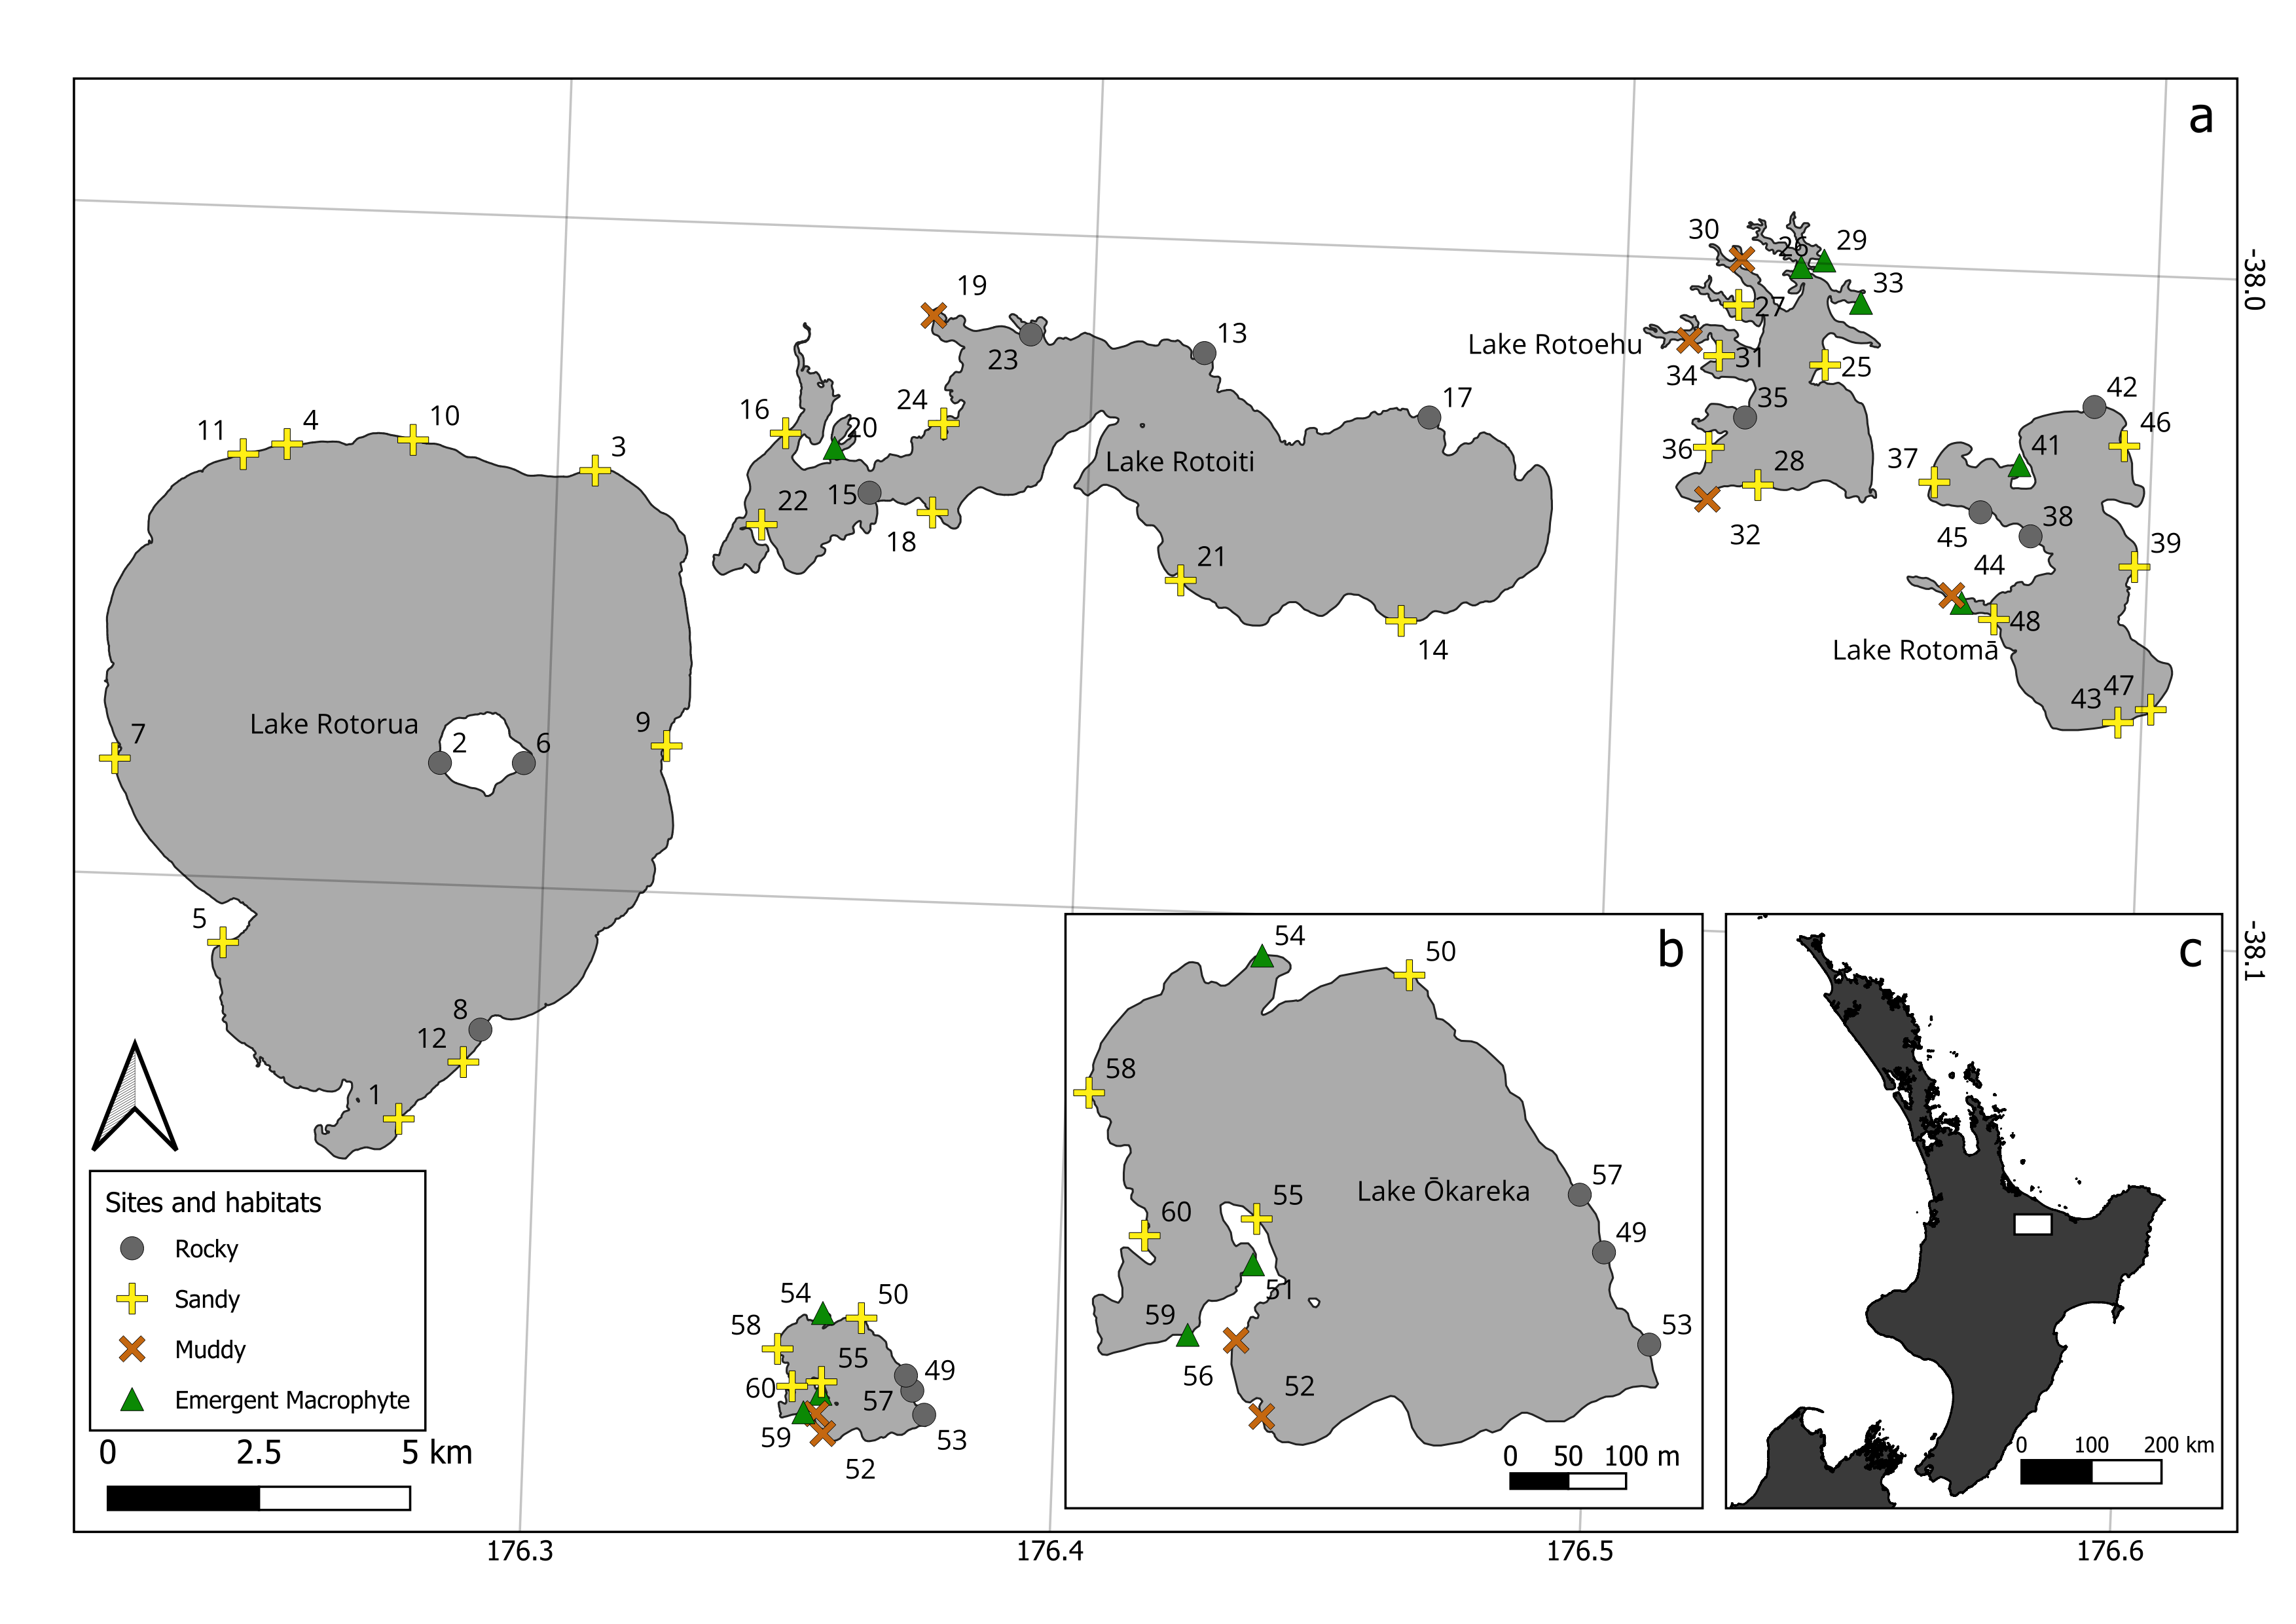
\includegraphics[keepaspectratio]{images/Natural_habitat_map.png}}

}

\caption{\label{fig-site-map}Map of the sampling locations with
different dominant littoral habitat types classified. a) Overview map of
the 5 lakes. Lakes where invasive catfish were detected are indicated.
b) Zoom in of Lake Ōkāreka. c) Guidance map to show the lakes location
(white square) on the North Island of Aotearoa New Zealand.}

\end{figure}%

\begin{figure}

\centering{


\includegraphics[width=3in,height=\textheight,keepaspectratio]{outputs/fig-koura-by-lake.png}

}

\caption{\label{fig-koura-by-lake}Kōura presence, CPUE, and BPUE across
lakes. The upper panel shows the proportion of sampled sites with kōura
present in each lake, with error bars indicating 95\% binomial
confidence intervals. The middle and lower panels show the distribution
of kōura CPUE and BPUE, respectively, across lakes using boxplots
(median, interquartile range, and range).}

\end{figure}%

\begin{figure}

\centering{

\includegraphics[width=6.5in,height=\textheight,keepaspectratio]{outputs/fig-occupancy-model.png}

}

\caption{\label{fig-occupancy-model}Kōura occupancy GAMM results and
model performance. a) Estimated smooth terms for riparian vegetation,
substrate index, surface water temperature, and specific conductivity,
shown as partial effects with 95\% confidence intervals. See Fig. S2 for
raw data underlying modelled relationships. b) Receiver operating
characteristic (ROC) curve illustrating model discrimination, with the
area under the curve (AUC) reported. c) Calibration plot based on five
equal-frequency bins, comparing mean predicted occupancy probabilities
with observed proportions of occupied sites; the dashed 1:1 line
indicates perfect calibration.}

\end{figure}%

\begin{figure}

\centering{

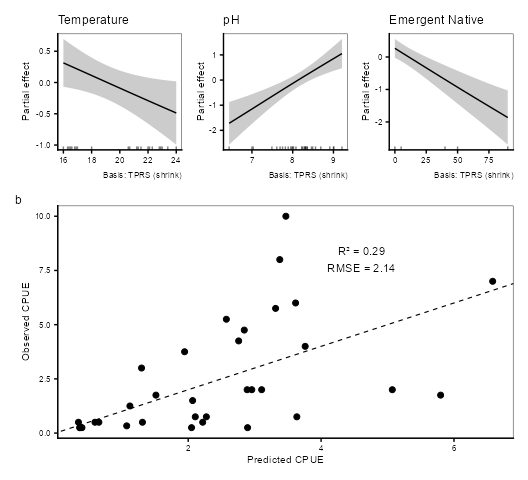
\includegraphics[width=5.5in,height=\textheight,keepaspectratio]{outputs/fig-cpue-hurdle.png}

}

\caption{\label{fig-cpue-hurdle}Kōura CPUE GAMM results and model
performance. a) Estimated smooth terms for surface water temperature,
pH, and emergent native macrophytes, shown with partial effects and 95\%
confidence intervals. See Fig. S2 for raw data underlying modelled
relationships. b) Predicted versus observed CPUE from the positive
(Gamma) component of the hurdle model, with predictions excluding the
random lake effect. The dashed 1:1 line indicates perfect agreement;
annotated values report R² and RMSE to summarise model fit.}

\end{figure}%

\begin{figure}

\centering{

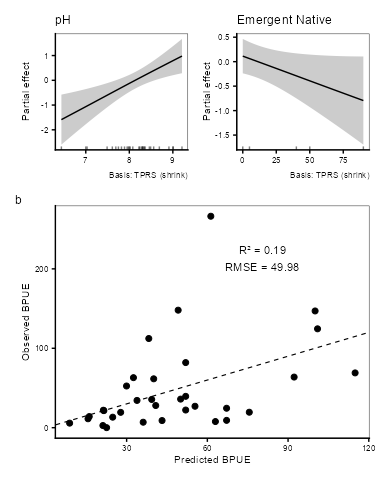
\includegraphics[width=4in,height=\textheight,keepaspectratio]{outputs/fig-bpue-hurdle.png}

}

\caption{\label{fig-bpue-hurdle}Kōura BPUE GAMM results and model
performance. a) Estimated smooth terms for pH and emergent native
macrophytes, shown with partial effects and 95\% confidence intervals.
See Fig. S2 for raw data underlying modelled relationships. b) Predicted
versus observed BPUE from the positive (Gamma) component of the hurdle
model, with predictions excluding the random lake effect. The dashed 1:1
line indicates perfect agreement; annotated values report R² and RMSE to
summarise model fit.}

\end{figure}%

\section{Supplementary information}\label{supplementary-information}

\begin{figure}

\centering{


\includegraphics[width=6.5in,height=\textheight,keepaspectratio]{outputs/fig-length-weight.png}

}

\caption{\label{fig-length-weight}Length--weight relationship used to
estimate missing kōura weights. Observed (measured) and model-predicted
body weights are shown in relation to orbital carapace length (OCL). The
log₁₀--log₁₀ regression was fitted to individuals with both length and
weight measurements (n = 240) and used to estimate missing weights (n =
81). Predicted values were back-transformed using a lognormal bias
correction factor. The fitted regression equation is shown on the plot.}

\end{figure}%

\begin{figure}

\centering{


\includegraphics[width=5in,height=\textheight,keepaspectratio]{outputs/fig-raw-data-all-predictors.png}

}

\caption{\label{fig-raw-data-all-predictors}Raw relationships between
all environmental predictors examined and kōura occurrence, CPUE, and
BPUE across all 60 surveyed littoral sites. Each panel shows observed
values at individual sites (n = 60 for occurrence; n = 33 for CPUE and
BPUE). Points are jittered slightly for occurrence data to reduce
overplotting. Predictors highlighted in bold were retained in final GAM
models.}

\end{figure}%

{

\begin{longtable}[]{@{}
  >{\raggedright\arraybackslash}p{(\linewidth - 18\tabcolsep) * \real{0.1149}}
  >{\raggedright\arraybackslash}p{(\linewidth - 18\tabcolsep) * \real{0.2529}}
  >{\raggedright\arraybackslash}p{(\linewidth - 18\tabcolsep) * \real{0.1034}}
  >{\raggedleft\arraybackslash}p{(\linewidth - 18\tabcolsep) * \real{0.0345}}
  >{\raggedleft\arraybackslash}p{(\linewidth - 18\tabcolsep) * \real{0.0805}}
  >{\raggedleft\arraybackslash}p{(\linewidth - 18\tabcolsep) * \real{0.0805}}
  >{\raggedleft\arraybackslash}p{(\linewidth - 18\tabcolsep) * \real{0.0805}}
  >{\raggedleft\arraybackslash}p{(\linewidth - 18\tabcolsep) * \real{0.0805}}
  >{\raggedleft\arraybackslash}p{(\linewidth - 18\tabcolsep) * \real{0.0805}}
  >{\raggedleft\arraybackslash}p{(\linewidth - 18\tabcolsep) * \real{0.0920}}@{}}

\caption{\label{tbl-env-fish-summary}Distribution of environmental and
biotic variables measured at littoral sampling sites across five Te
Arawa lakes in the Rotorua region of Aotearoa New Zealand.}

\tabularnewline

\toprule\noalign{}
\begin{minipage}[b]{\linewidth}\raggedright
Lake
\end{minipage} & \begin{minipage}[b]{\linewidth}\raggedright
Variable
\end{minipage} & \begin{minipage}[b]{\linewidth}\raggedright
Unit
\end{minipage} & \begin{minipage}[b]{\linewidth}\raggedleft
n
\end{minipage} & \begin{minipage}[b]{\linewidth}\raggedleft
Mean
\end{minipage} & \begin{minipage}[b]{\linewidth}\raggedleft
Median
\end{minipage} & \begin{minipage}[b]{\linewidth}\raggedleft
Min
\end{minipage} & \begin{minipage}[b]{\linewidth}\raggedleft
Max
\end{minipage} & \begin{minipage}[b]{\linewidth}\raggedleft
CI low
\end{minipage} & \begin{minipage}[b]{\linewidth}\raggedleft
CI high
\end{minipage} \\
\midrule\noalign{}
\endhead
\bottomrule\noalign{}
\endlastfoot
Rotorua & Substrate index & & 12 & 3.66 & 3.30 & 2.80 & 6.30 & 3.01 &
4.31 \\
Rotoiti & Substrate index & & 12 & 3.92 & 3.20 & 2.00 & 8.00 & 2.73 &
5.11 \\
Rotoehu & Substrate index & & 12 & 2.77 & 2.45 & 2.00 & 4.90 & 2.15 &
3.39 \\
Rotomā & Substrate index & & 12 & 3.50 & 3.03 & 2.00 & 6.20 & 2.64 &
4.36 \\
Ōkāreka & Substrate index & & 12 & 2.86 & 2.70 & 1.00 & 6.20 & 1.92 &
3.79 \\
All lakes & Substrate index & & 60 & 3.34 & 3.00 & 1.00 & 8.00 & 2.98 &
3.71 \\
Rotorua & Slope 5m & & 12 & 0.02 & 0.01 & 0.01 & 0.16 & 0.00 & 0.05 \\
Rotoiti & Slope 5m & & 12 & 0.09 & 0.07 & 0.04 & 0.30 & 0.04 & 0.14 \\
Rotoehu & Slope 5m & & 12 & 0.08 & 0.06 & 0.02 & 0.27 & 0.03 & 0.12 \\
Rotomā & Slope 5m & & 12 & 0.07 & 0.06 & 0.01 & 0.23 & 0.03 & 0.11 \\
Ōkāreka & Slope 5m & & 12 & 0.11 & 0.13 & 0.01 & 0.20 & 0.07 & 0.15 \\
All lakes & Slope 5m & & 60 & 0.08 & 0.06 & 0.01 & 0.30 & 0.06 & 0.09 \\
Rotorua & Riparian vegetation & \% & 12 & 67.50 & 100.00 & 0.00 & 100.00
& 40.12 & 94.88 \\
Rotoiti & Riparian vegetation & \% & 12 & 92.50 & 100.00 & 20.00 &
100.00 & 77.88 & 107.12 \\
Rotoehu & Riparian vegetation & \% & 12 & 67.50 & 100.00 & 0.00 & 100.00
& 36.95 & 98.05 \\
Rotomā & Riparian vegetation & \% & 12 & 63.33 & 90.00 & 0.00 & 100.00 &
35.13 & 91.53 \\
Ōkāreka & Riparian vegetation & \% & 12 & 75.83 & 100.00 & 0.00 & 100.00
& 48.01 & 103.66 \\
All lakes & Riparian vegetation & \% & 60 & 73.33 & 100.00 & 0.00 &
100.00 & 62.65 & 84.02 \\
Rotorua & Overhanging trees & \% & 12 & 46.67 & 30.00 & 0.00 & 100.00 &
15.50 & 77.83 \\
Rotoiti & Overhanging trees & \% & 12 & 54.17 & 65.00 & 0.00 & 100.00 &
23.22 & 85.11 \\
Rotoehu & Overhanging trees & \% & 12 & 35.83 & 0.00 & 0.00 & 100.00 &
5.25 & 66.42 \\
Rotomā & Overhanging trees & \% & 12 & 52.50 & 55.00 & 0.00 & 100.00 &
22.44 & 82.56 \\
Ōkāreka & Overhanging trees & \% & 12 & 52.50 & 65.00 & 0.00 & 100.00 &
21.71 & 83.29 \\
All lakes & Overhanging trees & \% & 60 & 48.33 & 30.00 & 0.00 & 100.00
& 36.15 & 60.52 \\
Rotorua & Wood cover & \% & 12 & 8.33 & 3.50 & 0.00 & 30.00 & 1.98 &
14.69 \\
Rotoiti & Wood cover & \% & 12 & 4.25 & 1.50 & 0.00 & 20.00 & 0.31 &
8.19 \\
Rotoehu & Wood cover & \% & 12 & 14.92 & 10.00 & 3.00 & 40.00 & 7.24 &
22.60 \\
Rotomā & Wood cover & \% & 12 & 10.00 & 10.00 & 0.00 & 30.00 & 4.13 &
15.87 \\
Ōkāreka & Wood cover & \% & 12 & 11.25 & 7.50 & 0.00 & 40.00 & 2.56 &
19.94 \\
All lakes & Wood cover & \% & 60 & 9.75 & 5.00 & 0.00 & 40.00 & 6.96 &
12.54 \\
Rotorua & Emergent macrophytes & \% & 12 & 0.00 & 0.00 & 0.00 & 0.00 &
0.00 & 0.00 \\
Rotoiti & Emergent macrophytes & \% & 12 & 9.50 & 0.00 & 0.00 & 100.00 &
-8.71 & 27.71 \\
Rotoehu & Emergent macrophytes & \% & 12 & 8.75 & 0.00 & 0.00 & 35.00 &
-0.74 & 18.24 \\
Rotomā & Emergent macrophytes & \% & 12 & 10.83 & 0.00 & 0.00 & 80.00 &
-4.78 & 26.45 \\
Ōkāreka & Emergent macrophytes & \% & 12 & 22.50 & 0.00 & 0.00 & 90.00 &
-0.35 & 45.35 \\
All lakes & Emergent macrophytes & \% & 60 & 10.32 & 0.00 & 0.00 &
100.00 & 3.98 & 16.65 \\
Rotorua & Submerged macrophytes & \% & 12 & 0.83 & 0.00 & 0.00 & 10.00 &
-1.00 & 2.67 \\
Rotoiti & Submerged macrophytes & \% & 12 & 0.83 & 0.00 & 0.00 & 10.00 &
-1.00 & 2.67 \\
Rotoehu & Submerged macrophytes & \% & 12 & 51.42 & 52.50 & 0.00 &
100.00 & 20.51 & 82.33 \\
Rotomā & Submerged macrophytes & \% & 12 & 21.67 & 10.00 & 0.00 & 85.00
& 2.21 & 41.12 \\
Ōkāreka & Submerged macrophytes & \% & 12 & 10.83 & 0.00 & 0.00 & 100.00
& -7.43 & 29.10 \\
All lakes & Submerged macrophytes & \% & 60 & 17.12 & 0.00 & 0.00 &
100.00 & 8.42 & 25.81 \\
Rotorua & Temperature & Degree C & 12 & 23.15 & 23.25 & 21.80 & 25.30 &
22.52 & 23.78 \\
Rotoiti & Temperature & Degree C & 12 & 21.62 & 21.50 & 20.60 & 23.80 &
21.03 & 22.22 \\
Rotoehu & Temperature & Degree C & 12 & 22.11 & 22.05 & 21.20 & 23.00 &
21.72 & 22.49 \\
Rotomā & Temperature & Degree C & 12 & 17.02 & 16.85 & 16.30 & 18.10 &
16.64 & 17.39 \\
Ōkāreka & Temperature & Degree C & 12 & 16.98 & 16.30 & 16.00 & 20.70 &
15.93 & 18.04 \\
All lakes & Temperature & Degree C & 60 & 20.18 & 21.25 & 16.00 & 25.30
& 19.44 & 20.91 \\
Rotorua & Dissolved oxygen & mg/l & 12 & 8.49 & 7.92 & 5.25 & 11.05 &
7.39 & 9.59 \\
Rotoiti & Dissolved oxygen & mg/l & 12 & 9.59 & 9.75 & 6.80 & 10.64 &
8.92 & 10.25 \\
Rotoehu & Dissolved oxygen & mg/l & 12 & 10.36 & 10.77 & 8.85 & 11.79 &
9.67 & 11.05 \\
Rotomā & Dissolved oxygen & mg/l & 12 & 9.72 & 9.76 & 8.66 & 10.31 &
9.45 & 9.98 \\
Ōkāreka & Dissolved oxygen & mg/l & 12 & 9.37 & 9.38 & 8.83 & 9.74 &
9.20 & 9.53 \\
All lakes & Dissolved oxygen & mg/l & 60 & 9.50 & 9.62 & 5.25 & 11.79 &
9.20 & 9.81 \\
Rotorua & Specific conductivity & µS/cm & 12 & 205.36 & 188.27 & 156.20
& 443.01 & 156.39 & 254.33 \\
Rotoiti & Specific conductivity & µS/cm & 12 & 163.11 & 158.70 & 155.79
& 196.01 & 156.22 & 170.00 \\
Rotoehu & Specific conductivity & µS/cm & 12 & 458.89 & 458.22 & 455.44
& 464.72 & 456.91 & 460.87 \\
Rotomā & Specific conductivity & µS/cm & 12 & 162.90 & 161.79 & 156.73 &
174.96 & 159.94 & 165.85 \\
Ōkāreka & Specific conductivity & µS/cm & 12 & 76.34 & 76.15 & 75.62 &
78.59 & 75.82 & 76.86 \\
All lakes & Specific conductivity & µS/cm & 60 & 213.32 & 162.55 & 75.62
& 464.72 & 178.41 & 248.23 \\
Rotorua & pH & & 12 & 6.94 & 7.04 & 3.78 & 7.69 & 6.29 & 7.60 \\
Rotoiti & pH & & 12 & 8.67 & 8.73 & 8.08 & 9.02 & 8.46 & 8.87 \\
Rotoehu & pH & & 12 & 8.83 & 8.91 & 8.46 & 9.21 & 8.68 & 8.99 \\
Rotomā & pH & & 12 & 7.80 & 7.92 & 6.44 & 8.56 & 7.47 & 8.13 \\
Ōkāreka & pH & & 12 & 8.32 & 8.29 & 7.77 & 9.00 & 8.15 & 8.50 \\
All lakes & pH & & 60 & 8.11 & 8.28 & 3.78 & 9.21 & 7.89 & 8.34 \\
Rotorua & Presence Catfish & & 12 & 0.08 & 0.00 & 0.00 & 1.00 & 0.00 &
0.38 \\
Rotoiti & Presence Catfish & & 12 & 0.42 & 0.00 & 0.00 & 1.00 & 0.15 &
0.72 \\
Rotoehu & Presence Catfish & & 12 & 0.00 & 0.00 & 0.00 & 0.00 & 0.00 &
0.26 \\
Rotomā & Presence Catfish & & 12 & 0.00 & 0.00 & 0.00 & 0.00 & 0.00 &
0.26 \\
Ōkāreka & Presence Catfish & & 12 & 0.00 & 0.00 & 0.00 & 0.00 & 0.00 &
0.26 \\
All lakes & Presence Catfish & & 60 & 0.10 & 0.00 & 0.00 & 1.00 & 0.04 &
0.21 \\
Rotorua & Presence Eel & & 12 & 0.33 & 0.00 & 0.00 & 1.00 & 0.10 &
0.65 \\
Rotoiti & Presence Eel & & 12 & 0.08 & 0.00 & 0.00 & 1.00 & 0.00 &
0.38 \\
Rotoehu & Presence Eel & & 12 & 0.00 & 0.00 & 0.00 & 0.00 & 0.00 &
0.26 \\
Rotomā & Presence Eel & & 12 & 0.25 & 0.00 & 0.00 & 1.00 & 0.05 &
0.57 \\
Ōkāreka & Presence Eel & & 12 & 0.00 & 0.00 & 0.00 & 0.00 & 0.00 &
0.26 \\
All lakes & Presence Eel & & 60 & 0.13 & 0.00 & 0.00 & 1.00 & 0.06 &
0.25 \\
Rotorua & Presence Goldfish & & 12 & 0.08 & 0.00 & 0.00 & 1.00 & 0.00 &
0.38 \\
Rotoiti & Presence Goldfish & & 12 & 0.67 & 1.00 & 0.00 & 1.00 & 0.35 &
0.90 \\
Rotoehu & Presence Goldfish & & 12 & 1.00 & 1.00 & 1.00 & 1.00 & 0.74 &
1.00 \\
Rotomā & Presence Goldfish & & 12 & 0.50 & 0.50 & 0.00 & 1.00 & 0.21 &
0.79 \\
Ōkāreka & Presence Goldfish & & 12 & 0.25 & 0.00 & 0.00 & 1.00 & 0.05 &
0.57 \\
All lakes & Presence Goldfish & & 60 & 0.50 & 0.50 & 0.00 & 1.00 & 0.37
& 0.63 \\
Rotorua & Presence Common smelt & & 12 & 0.25 & 0.00 & 0.00 & 1.00 &
0.05 & 0.57 \\
Rotoiti & Presence Common smelt & & 12 & 0.67 & 1.00 & 0.00 & 1.00 &
0.35 & 0.90 \\
Rotoehu & Presence Common smelt & & 12 & 0.50 & 0.50 & 0.00 & 1.00 &
0.21 & 0.79 \\
Rotomā & Presence Common smelt & & 12 & 0.42 & 0.00 & 0.00 & 1.00 & 0.15
& 0.72 \\
Ōkāreka & Presence Common smelt & & 12 & 0.58 & 1.00 & 0.00 & 1.00 &
0.28 & 0.85 \\
All lakes & Presence Common smelt & & 60 & 0.48 & 0.00 & 0.00 & 1.00 &
0.35 & 0.62 \\
Rotorua & Presence Kōaro & & 12 & 0.00 & 0.00 & 0.00 & 0.00 & 0.00 &
0.26 \\
Rotoiti & Presence Kōaro & & 12 & 0.00 & 0.00 & 0.00 & 0.00 & 0.00 &
0.26 \\
Rotoehu & Presence Kōaro & & 12 & 0.00 & 0.00 & 0.00 & 0.00 & 0.00 &
0.26 \\
Rotomā & Presence Kōaro & & 12 & 0.00 & 0.00 & 0.00 & 0.00 & 0.00 &
0.26 \\
Ōkāreka & Presence Kōaro & & 12 & 0.67 & 1.00 & 0.00 & 1.00 & 0.35 &
0.90 \\
All lakes & Presence Kōaro & & 60 & 0.13 & 0.00 & 0.00 & 1.00 & 0.06 &
0.25 \\
Rotorua & Presence Trout & & 12 & 0.17 & 0.00 & 0.00 & 1.00 & 0.02 &
0.48 \\
Rotoiti & Presence Trout & & 12 & 0.17 & 0.00 & 0.00 & 1.00 & 0.02 &
0.48 \\
Rotoehu & Presence Trout & & 12 & 0.00 & 0.00 & 0.00 & 0.00 & 0.00 &
0.26 \\
Rotomā & Presence Trout & & 12 & 0.00 & 0.00 & 0.00 & 0.00 & 0.00 &
0.26 \\
Ōkāreka & Presence Trout & & 12 & 0.17 & 0.00 & 0.00 & 1.00 & 0.02 &
0.48 \\
All lakes & Presence Trout & & 60 & 0.10 & 0.00 & 0.00 & 1.00 & 0.04 &
0.21 \\

\end{longtable}

}

\protect\phantomsection\label{refs}
\begin{CSLReferences}{0}{1}
\bibitem[\citeproctext]{ref-Albertson2018}
Albertson, L. K., \& M. D. Daniels, 2018. Crayfish ecosystem engineering
effects on riverbed disturbance and topography are mediated by size and
behavior. Freshwater Science 37: 836--844.
\url{https://doi.org/10.1086/700884}.

\bibitem[\citeproctext]{ref-Angilletta2004}
Angilletta, M. J., T. D. Steury, \& M. W. Sears, 2004. Temperature,
growth rate, and body size in ectotherms: Fitting pieces of a
life-history puzzle. Integrative and Comparative Biology 44: 498--509.
\url{https://doi.org/10.1093/icb/44.6.498}.

\bibitem[\citeproctext]{ref-Barnes1996}
Barnes, G. E., 1996.
\href{https://researchcommons.waikato.ac.nz/items/24cf02c1-8c2f-4b63-ba89-e8a509e9ba05}{The
biology and general ecology of the brown bullhead catfish
({\emph{Ameiurus nebulosus}}) in {Lake Taupo}}. Master of Science
thesis, University of Waikato.

\bibitem[\citeproctext]{ref-Barnes2003}
Barnes, G. E., \& B. J. Hicks, 2003. Brown bullhead catfish
({\emph{Ameiurus nebulosus}}) in {Lake Taupo}. In Managing invasive
freshwater fish in {New Zealand}: Proceedings of a workshop hosted by
{Department of Conservation}, 10-12 may 2001, {Hamilton}. Department of
Conservation.

\bibitem[\citeproctext]{ref-Bolker2009}
Bolker, B. M., M. E. Brooks, C. J. Clark, S. W. Geange, J. R. Poulsen,
M. H. H. Stevens, \& J.-S. S. White, 2009. Generalized linear mixed
models: A practical guide for ecology and evolution. Trends in Ecology
\& Evolution 24: 127--135.
\url{https://doi.org/10.1016/j.tree.2008.10.008}.

\bibitem[\citeproctext]{ref-Brooks2017}
Brooks, M., B. Bolker, K. Kristensen, M. Maechler, A. Magnusson, H.
Skaug, A. Nielsen, C. Berg, \& K. van Bentham, 2017.
\href{https://doi.org/10.32614/cran.package.glmmtmb}{glmmTMB:
Generalized linear mixed models using template model builder}.

\bibitem[\citeproctext]{ref-Broughton2017}
Broughton, R. J., I. D. Marsden, J. V. Hill, \& C. N. Glover, 2017.
Behavioural, physiological and biochemical responses to aquatic hypoxia
in the freshwater crayfish, {\emph{Paranephrops zealandicus}}.
Comparative Biochemistry and Physiology Part A: Molecular \& Integrative
Physiology 212: 72--80.
\url{https://doi.org/10.1016/j.cbpa.2017.07.013}.

\bibitem[\citeproctext]{ref-Bunch2010}
Bunch, A. J., M. S. Allen, \& D. C. Gwinn, 2010. Spatial and temporal
hypoxia dynamics in dense emergent macrophytes in a {Florida} lake.
Wetlands 30: 429--435. \url{https://doi.org/10.1007/s13157-010-0051-9}.

\bibitem[\citeproctext]{ref-Capinha2013}
Capinha, C., E. R. Larson, E. Tricarico, J. D. Olden, \& F. Gherardi,
2013. Effects of climate change, invasive species, and disease on the
distribution of native {European} crayfishes. Conservation Biology 27:
731--740. \url{https://doi.org/10.1111/cobi.12043}.

\bibitem[\citeproctext]{ref-Chambers1987}
Chambers, P. A., 1987. Nearshore occurrence of submersed aquatic
macrophytes in relation to wave action. Canadian Journal of Fisheries
and Aquatic Sciences 44: 1666--1669.
\url{https://doi.org/10.1139/f87-204}.

\bibitem[\citeproctext]{ref-Coffey1988}
Coffey, B. T., \& J. S. Clayton, 1988. Contrasting deep-water macrophyte
communities in two highly transparent {New Zealand} lakes and their
possible association with freshwater crayfish, {\emph{Paranephrops}}
spp. New Zealand Journal of Marine and Freshwater Research 22: 225--230.
\url{https://doi.org/10.1080/00288330.1988.9516294}.

\bibitem[\citeproctext]{ref-Collier1997}
Collier, K. J., S. M. Parkyn, \& C. F. Rabeni, 1997. Koura: A keystone
species. Water and Atmosphere 5: 18--20.

\bibitem[\citeproctext]{ref-Creed2004}
Creed, R. P., \& J. M. Reed, 2004. Ecosystem engineering by crayfish in
a headwater stream community. Journal of the North American
Benthological Society 23: 224--236.
\url{https://doi.org/10.1899/0887-3593(2004)023\%3C0224:EEBCIA\%3E2.0.CO;2}.

\bibitem[\citeproctext]{ref-Danilovic2022}
Danilović, M., I. Maguire, \& L. Füreder, 2022. Overlooked keystone
species in conservation plans of fluvial ecosystems in {Southeast
Europe}: A review of native freshwater crayfish species. Knowledge \&
Management of Aquatic Ecosystems 423: 21.
\url{https://doi.org/10.1051/kmae/2022016}.

\bibitem[\citeproctext]{ref-Dedual2002}
Dedual, M., 2002. Vertical distribution and movements of brown bullhead
({\emph{Ameiurus nebulosus}} {Lesueur} 1819) in {Motuoapa Bay}, southern
{Lake Taupo}, {New Zealand}. Hydrobiologia 483: 129--135.
\url{https://doi.org/10.1007/978-94-017-0771-8_15}.

\bibitem[\citeproctext]{ref-Devcich1979}
Devcich, A. A., 1979. An ecological study of {\emph{Paranephrops
planifrons}} {White} ({Decapoda}: {Parastacidae}) in {Lake Rotoiti},
{North Island}. PhD thesis, University of Waikato.

\bibitem[\citeproctext]{ref-Dumelle2023}
Dumelle, M., T. Kincaid, A. R. Olsen, \& M. Weber, 2023. Spsurvey:
Spatial sampling design and analysis in {R}. Journal of Statistical
Software 105: \url{https://doi.org/10.18637/jss.v105.i03}.

\bibitem[\citeproctext]{ref-Fielding1997}
Fielding, A. H., \& J. F. Bell, 1997. A review of methods for the
assessment of prediction errors in conservation presence/absence models.
Environmental Conservation 24: 38--49.
\url{https://doi.org/10.1017/S0376892997000088}.

\bibitem[\citeproctext]{ref-Ford2005}
Ford, T., \& T. L. Beitinger, 2005. Temperature tolerance in the
goldfish, {\emph{Carassius auratus}}. Journal of Thermal Biology 30:
147--152. \url{https://doi.org/10.1016/j.jtherbio.2004.09.004}.

\bibitem[\citeproctext]{ref-Francis2019}
Francis, L. B., 2019.
\href{https://researchcommons.waikato.ac.nz/handle/10289/12746}{Evaluating
the effects of invasive brown bullhead catfish ({\emph{Ameiurus
nebulosus}}) on k{ō}ura (freshwater crayfish, {\emph{Paranephrops
planifrons}}) in {Lake Rotoiti}}. Master's thesis, University of
Waikato.

\bibitem[\citeproctext]{ref-Froese2006}
Froese, R., 2006. Cube law, condition factor and weight-length
relationships: History, meta-analysis and recommendations. Journal of
Applied Ichthyology 22: 241--253.
\url{https://doi.org/10.1111/j.1439-0426.2006.00805.x}.

\bibitem[\citeproctext]{ref-Fry1948}
Fry, F. E. J., \& J. S. Hart, 1948. Cruising speed of goldfish in
relation to water temperature. Journal of the Fisheries Research Board
of Canada 7b: 169--175. \url{https://doi.org/10.1139/f47-018}.

\bibitem[\citeproctext]{ref-Grayling2020}
Grayling, S., 2020.
\href{https://atlas.boprc.govt.nz/api/v1/edms/document/A3651696/content}{{Bay
of Plenty} regional pest management plan 2011-2016 annual report for
2019/2020}. Bay of Plenty Regional Council.

\bibitem[\citeproctext]{ref-Greenaway1985}
Greenaway, P., 1985. Calcium balance and moulting in the {Crustacea}.
Biological Reviews 60: 425--454.

\bibitem[\citeproctext]{ref-Hamilton2005}
Hamilton, D., C. McBride, \& T. Uraoka, 2005. {Lake Rotoiti} fieldwork
and modelling to support considerations of {Ohau} channel diversion from
{Lake Rotoiti}. NIWA \& University of Waikato.

\bibitem[\citeproctext]{ref-Hammond2006}
Hammond, K. S., J. W. Hollows, C. R. Townsend, \& P. M. Lokman, 2006.
Effects of temperature and water calcium concentration on growth,
survival and moulting of freshwater crayfish, {\emph{Paranephrops
zealandicus}}. Aquaculture 251: 271--279.
\url{https://doi.org/10.1016/j.aquaculture.2005.05.032}.

\bibitem[\citeproctext]{ref-Harding2009}
Harding, J. S., J. E. Clapcott, J. M. Quinn, J. W. Hayes, M. K. Joy, R.
G. Storey, H. S. Greig, J. Hay, T. James, M. A. Beech, R. Ozane, A. S.
Meredith, \& I. K. G. Boothroyd, 2009. Stream habitat assessment
protocols for wadeable rivers and streams of {New Zealand}. School of
Biological Sciences, University of Canterbury.

\bibitem[\citeproctext]{ref-Haschenburger2009}
Haschenburger, J. K., \& P. Roest, 2009. Substrate indices as indicators
of interstitial pore space in gravel-bed channels. River Research and
Applications 25: 98--105. \url{https://doi.org/10.1002/rra.1168}.

\bibitem[\citeproctext]{ref-Hesni2009}
Hesni, M. A., N. Shabanipour, A. Zahmatkesh, \& M. M. Toutouni, 2009.
Effects of temperature and salinity on survival and moulting of the
narrow-clawed crayfish, {\emph{Astacus leptodactylus}} {Eschscholtz},
1823 ({Decapoda}, {Astacidea}). Crustaceana 82: 1495--1507.
\url{https://doi.org/10.1163/156854009X407191}.

\bibitem[\citeproctext]{ref-Hessen2004}
Hessen, D. O., J. Skurdal, \& J. E. Braathen, 2004. Plant exclusion of a
herbivore; crayfish population decline caused by an invading waterweed.
Biological Invasions 6: 133--140.
\url{https://doi.org/10.1023/B:BINV.0000022131.40783.f0}.

\bibitem[\citeproctext]{ref-Hiroa1921}
Hiroa, T. R., 1921. M{ā}ori food-supplies of {Lake Rotorua}, with
methods of obtaining them, and usages and customs appertaining thereto.
Transactions and Proceedings of the Royal Society of New Zealand
1868-1961 53: 433--451.

\bibitem[\citeproctext]{ref-Hopkins1970}
Hopkins, C. L., 1970. Systematics of the {New Zealand} freshwater
crayfish {\emph{Paranephrops}} ({Crustacea}: {Decapoda}:
{Parastacidae}). New Zealand Journal of Marine and Freshwater Research
4: 278--291. \url{https://doi.org/10.1080/00288330.1970.9515347}.

\bibitem[\citeproctext]{ref-Jane2021}
{Jane, S. F., G. J. A. Hansen, B. M. Kraemer, P. R. Leavitt, J. L.
Mincer, R. L. North, R. M. Pilla, J. T. Stetler, C. E. Williamson, R. I.
Woolway, \& others}, 2021. Widespread deoxygenation of temperate lakes.
Nature 594: 66--70. \url{https://doi.org/10.1038/s41586-021-03550-y}.

\bibitem[\citeproctext]{ref-Johnsen2008}
Johnsen, S. I., \& T. Taugbøl, 2008. Add stones, get crayfish - is it
that simple? Freshwater Crayfish 16: 47--50.

\bibitem[\citeproctext]{ref-Jowett2008}
Jowett, I. G., S. M. Parkyn, \& J. Richardson, 2008. Habitat
characteristics of crayfish ({\emph{Paranephrops planifrons}}) in {New
Zealand} streams using generalised additive models ({GAMs}).
Hydrobiologia 596: 353--365.
\url{https://doi.org/10.1007/s10750-007-9108-z}.

\bibitem[\citeproctext]{ref-Jowett1990}
Jowett, I. G., \& J. Richardson, 1990. Microhabitat preferences of
benthic invertebrates in a {New Zealand} river and the development of
in-stream flow-habitat models for {\emph{Deleatidium}} spp. New Zealand
Journal of Marine and Freshwater Research 24: 19--30.
\url{https://doi.org/10.1080/00288330.1990.9516399}.

\bibitem[\citeproctext]{ref-Kusabs2026}
Kusabs, I. A. K., I. C. Duggan, A. C. Bruere, P. Scholes, T. W. Te
Kurapa, T. M. Grant, \& F. J. Burdon, 2026. Invasive catfish linked to
the decline of freshwater crayfish in two {Aotearoa New Zealand} lakes.
Biological Invasions 28:
\url{https://doi.org/10.1007/s10530-026-03852-0}.

\bibitem[\citeproctext]{ref-Kusabs2015a}
Kusabs, I. A., B. J. Hicks, J. M. Quinn, \& D. P. Hamilton, 2015a.
Sustainable management of freshwater crayfish (k{ō}ura,
{\emph{Paranephrops planifrons}}) in {Te Arawa} ({Rotorua}) lakes,
{North Island, New Zealand}. Fisheries Research 168: 35--46.
\url{https://doi.org/10.1016/j.fishres.2015.03.015}.

\bibitem[\citeproctext]{ref-Kusabs2009}
Kusabs, I. A., \& J. M. Quinn, 2009. Use of a traditional {Māori}
harvesting method, the tau k{ō}ura, for monitoring k{ō}ura (freshwater
crayfish, {\emph{Paranephrops planifrons}}) in {Lake Rotoiti}, {North
Island, New Zealand}. New Zealand Journal of Marine and Freshwater
Research 43: 713--722. \url{https://doi.org/10.1080/00288330909510036}.

\bibitem[\citeproctext]{ref-Kusabs2015b}
Kusabs, I. A., J. M. Quinn, \& D. P. Hamilton, 2015b. Effects of benthic
substrate, nutrient enrichment and predatory fish on freshwater crayfish
(k{ō}ura, {\emph{Paranephrops planifrons}}) population characteristics
in seven {Te Arawa} ({Rotorua}) lakes, {North Island, New Zealand}.
Marine and Freshwater Research 66: 631--643.
\url{https://doi.org/10.1071/MF14148}.

\bibitem[\citeproctext]{ref-Kutner2005}
Kutner, M. H., C. J. Nachtsheim, J. Neter, \& W. Li, 2005. Applied
linear statistical models. McGraw-Hill Irwin.

\bibitem[\citeproctext]{ref-LAWA2025}
Land, Air, Water Aotearoa (LAWA), 2025. Lakes data for the {Bay of
Plenty} region.
\url{https://www.lawa.org.nz/explore-data/bay-of-plenty-region/lakes}.

\bibitem[\citeproctext]{ref-Lee2025}
Lee, F., I. A. K. Kusabs, G. L. W. Perry, \& C. MacNeil, 2025.
Identifying refugia from the synergistic threats of climate change and
invasive species. Web Ecology 25: 221--239.
\url{https://doi.org/10.5194/we-25-221-2025}.

\bibitem[\citeproctext]{ref-Levin1992}
Levin, S. A., 1992. The problem of pattern and scale in ecology: The
{Robert H. MacArthur} award lecture. Ecology 73: 1943--1967.
\url{https://doi.org/10.2307/1941447}.

\bibitem[\citeproctext]{ref-Lishawa2023}
Lishawa, S. C., A. J. Schrank, B. A. Lawrence, A. M. Monks, \& D. A.
Albert, 2023. Aquatic connectivity treatments increase fish and
macroinvertebrate use of {\emph{Typha}}-invaded {Great Lakes} coastal
wetlands. Freshwater Biology 68: 1462--1477.
\url{https://doi.org/10.1111/fwb.14141}.

\bibitem[\citeproctext]{ref-Meerhoff2022}
Meerhoff, M., \& M. de los Ángeles González-Sagrario, 2022. Habitat
complexity in shallow lakes and ponds: Importance, threats, and
potential for restoration. Hydrobiologia 849: 3737--3760.
\url{https://doi.org/10.1007/s10750-021-04771-y}.

\bibitem[\citeproctext]{ref-Momot1995}
Momot, W. T., 1995. Redefining the role of crayfish in aquatic
ecosystems. Reviews in Fisheries Science 3: 33--63.
\url{https://doi.org/10.1080/10641269509388566}.

\bibitem[\citeproctext]{ref-Nystrom2006}
Nyström, P., P. Stenroth, N. Holmqvist, O. Berglund, P. Larsson, \& W.
Granéli, 2006. Crayfish in lakes and streams: Individual and population
responses to predation, productivity and substratum availability.
Freshwater Biology 51: 2096--2113.
\url{https://doi.org/10.1111/j.1365-2427.2006.01641.x}.

\bibitem[\citeproctext]{ref-Olsson2006}
Olsson, K., P. Stenroth, P. Nyström, N. Holmqvist, A. R. McIntosh, \& M.
J. Winterbourn, 2006. Does natural acidity mediate interactions between
introduced brown trout, native fish, crayfish and other invertebrates in
{West Coast New Zealand} streams? Biological Conservation 130: 255--267.
\url{https://doi.org/10.1016/j.biocon.2005.12.019}.

\bibitem[\citeproctext]{ref-Parkyn2002}
Parkyn, S. M., \& K. J. Collier, 2002. Differentiating the effects of
diet and temperature on juvenile crayfish ({\emph{Paranephrops
planifrons}}) growth: Leaf detritus versus invertebrate food sources at
two diurnally varying temperatures. Freshwater Crayfish 13: 371--382.

\bibitem[\citeproctext]{ref-Parkyn2004}
Parkyn, S. M., \& K. J. Collier, 2004. Interaction of press and pulse
disturbance on crayfish populations: Flood impacts in pasture and forest
streams. Hydrobiologia 527: 113--124.
\url{https://doi.org/10.1023/B:HYDR.0000043189.91134.94}.

\bibitem[\citeproctext]{ref-Parkyn2001}
Parkyn, S. M., K. J. Collier, \& B. J. Hicks, 2001. {New Zealand} stream
crayfish: Functional omnivores but trophic predators? Freshwater Biology
46: 641--652. \url{https://doi.org/10.1046/j.1365-2427.2001.00702.x}.

\bibitem[\citeproctext]{ref-Parkyn2009}
Parkyn, S. M., M. A. Meleason, \& R. J. Davies-Colley, 2009. Wood
enhances crayfish ({\emph{Paranephrops planifrons}}) habitat in a
forested stream. New Zealand Journal of Marine and Freshwater Research
43: 689--700. \url{https://doi.org/10.1080/00288330909510034}.

\bibitem[\citeproctext]{ref-Quinn2002}
Quinn, G. P., \& M. J. Keough, 2002. Experimental design and data
analysis for biologists. Cambridge University Press.

\bibitem[\citeproctext]{ref-Quinn1990}
Quinn, J. M., \& C. W. Hickey, 1990. Magnitude of effects of substrate
particle size, recent flooding, and catchment development on benthic
invertebrates in 88 {New Zealand} rivers. New Zealand Journal of Marine
and Freshwater Research 24: 411--427.
\url{https://doi.org/10.1080/00288330.1990.9516433}.

\bibitem[\citeproctext]{ref-RCoreTeam2025}
R Core Team, 2025. \href{https://www.R-project.org/}{{R}: A language and
environment for statistical computing}. R Foundation for Statistical
Computing, Vienna, Austria.

\bibitem[\citeproctext]{ref-Richman2015}
{Richman, N. I., M. Böhm, S. B. Adams, F. Alvarez, E. A. Bergey, J. J.
S. Bunn, Q. Burnham, J. Cordeiro, J. Coughran, K. A. Crandall, \&
others}, 2015. Multiple drivers of decline in the global status of
freshwater crayfish ({Decapoda}: {Astacidea}). Philosophical
Transactions of the Royal Society B: Biological Sciences 370: 20140060.
\url{https://doi.org/10.1098/rstb.2014.0060}.

\bibitem[\citeproctext]{ref-Rosewarne2013}
Rosewarne, P., A. Piper, R. Wright, \& A. Dunn, 2013. Do low-head
riverine structures hinder the spread of invasive crayfish? Case study
of signal crayfish ({\emph{Pacifastacus leniusculus}}) movements at a
flow gauging weir. Management of Biological Invasions 4: 273--282.
\url{https://doi.org/10.3391/mbi.2013.4.4.02}.

\bibitem[\citeproctext]{ref-Rowe1993}
Rowe, D. K., 1993. Identification of fish responsible for five layers of
echoes recorded by high-frequency (200 kHz) echosounding in {Lake
Rotoiti}, {North Island, New Zealand}. New Zealand Journal of Marine and
Freshwater Research 27: 87--100.
\url{https://doi.org/10.1080/00288330.1993.9516548}.

\bibitem[\citeproctext]{ref-Schoen2015}
Schoen, E. R., D. A. Beauchamp, A. R. Buettner, \& N. C. Overman, 2015.
Temperature and depth mediate resource competition and apparent
competition between {\emph{Mysis diluviana}} and kokanee. Ecological
Applications 25: 1962--1975. \url{https://doi.org/10.1890/14-1822.1}.

\bibitem[\citeproctext]{ref-Schrank2019}
Schrank, A. J., \& S. C. Lishawa, 2019. Invasive cattail reduces fish
diversity and abundance in the emergent marsh of a {Great Lakes} coastal
wetland. Journal of Great Lakes Research 45: 1251--1259.
\url{https://doi.org/10.1016/j.jglr.2019.09.013}.

\bibitem[\citeproctext]{ref-Shave1994}
Shave, C. R., C. R. Townsend, \& T. A. Crowl, 1994. Anti-predator
behaviours of a freshwater crayfish ({\emph{Paranephrops zealandicus}})
to a native and an introduced predator. New Zealand Journal of Ecology
18: 1--10.

\bibitem[\citeproctext]{ref-Shono2008}
Shono, H., 2008. Application of the {Tweedie} distribution to zero-catch
data in {CPUE} analysis. Fisheries Research 93: 154--162.
\url{https://doi.org/10.1016/j.fishres.2008.03.006}.

\bibitem[\citeproctext]{ref-Smith1996}
Smith, G. R. T., M. A. Learner, F. M. Slater, \& J. Foster, 1996.
Habitat features important for the conservation of the native crayfish
{\emph{Austropotamobius pallipes}} in {Britain}. Biological Conservation
75: 239--246. \url{https://doi.org/10.1016/0006-3207(95)00073-9}.

\bibitem[\citeproctext]{ref-Statzner2003}
Statzner, B., O. Peltret, \& S. Tomanova, 2003. Crayfish as geomorphic
agents and ecosystem engineers: Effect of a biomass gradient on baseflow
and flood-induced transport of gravel and sand in experimental streams.
Freshwater Biology 48: 147--163.
\url{https://doi.org/10.1046/j.1365-2427.2003.00984.x}.

\bibitem[\citeproctext]{ref-Stevens2004}
Stevens, D. L., \& A. R. Olsen, 2004. Spatially balanced sampling of
natural resources. Journal of the American Statistical Association 99:
262--278. \url{https://doi.org/10.1198/016214504000000250}.

\bibitem[\citeproctext]{ref-Strayer2010}
Strayer, D. L., \& S. E. G. Findlay, 2010. Ecology of freshwater shore
zones. Aquatic Sciences 72: 127--163.
\url{https://doi.org/10.1007/s00027-010-0128-9}.

\bibitem[\citeproctext]{ref-Taylor2019}
Taylor, C. A., R. J. DiStefano, E. R. Larson, \& J. Stoeckel, 2019.
Towards a cohesive strategy for the conservation of the {United States}'
diverse and highly endemic crayfish fauna. Hydrobiologia 846: 39--58.
\url{https://doi.org/10.1007/s10750-019-04066-3}.

\bibitem[\citeproctext]{ref-Usio2000}
Usio, N., \& C. R. Townsend, 2000. Distribution of the {New Zealand}
crayfish ({\emph{Paranephrops zealandicus}}) in relation to stream
physico-chemistry, predatory fish, and invertebrate prey. New Zealand
Journal of Marine and Freshwater Research 34: 557--567.
\url{https://doi.org/10.1080/00288330.2000.9516957}.

\bibitem[\citeproctext]{ref-Usio2004}
Usio, N., \& C. R. Townsend, 2004. Roles of crayfish: Consequences of
predation and bioturbation for stream invertebrates. Ecology 85:
807--822. \url{https://doi.org/10.1890/02-0618}.

\bibitem[\citeproctext]{ref-Vedia2017}
Vedia, I., D. Galicia, E. Baquero, J. Oscoz, \& R. Miranda, 2017.
Environmental factors influencing the distribution and abundance of the
introduced signal crayfish in the north of {Iberian Peninsula}. Marine
and Freshwater Research 68: 900--908.
\url{https://doi.org/10.1071/MF16020}.

\bibitem[\citeproctext]{ref-Vincent1984}
Vincent, W. F., M. M. Gibbs, \& S. J. Dryden, 1984. Accelerated
eutrophication in a {New Zealand} lake: {Lake Rotoiti}, central {North
Island}. New Zealand Journal of Marine and Freshwater Research 18:
431--440. \url{https://doi.org/10.1080/00288330.1984.9516064}.

\bibitem[\citeproctext]{ref-vonWesternhagen2010}
Westernhagen, N. von, D. P. Hamilton, \& C. A. Pilditch, 2010. Temporal
and spatial variations in phytoplankton productivity in surface waters
of a warm-temperate, monomictic lake in {New Zealand}. Hydrobiologia
652: 57--70. \url{https://doi.org/10.1007/s10750-010-0318-4}.

\bibitem[\citeproctext]{ref-Wetzel2001}
Wetzel, R. G., 2001. Limnology: Lake and river ecosystems. Gulf
Professional Publishing.

\bibitem[\citeproctext]{ref-White2003}
White, J., \& K. Irvine, 2003. The use of littoral mesohabitats and
their macroinvertebrate assemblages in the ecological assessment of
lakes. Aquatic Conservation: Marine and Freshwater Ecosystems 13:
331--351. \url{https://doi.org/10.1002/aqc.586}.

\bibitem[\citeproctext]{ref-Wood2004}
Wood, S. N., 2004. Stable and efficient multiple smoothing parameter
estimation for generalized additive models. Journal of the American
Statistical Association 99: 673--686.
\url{https://doi.org/10.1198/016214504000000980}.

\bibitem[\citeproctext]{ref-Wood2017}
Wood, S. N., 2017.
\href{https://doi.org/10.1201/9781315370279}{Generalized additive
models: An introduction with {R}}. Chapman; Hall/CRC.

\bibitem[\citeproctext]{ref-Woolway2021}
{Woolway, R. I., S. Sharma, G. A. Weyhenmeyer, A. Debolskiy, M. Golub,
D. Mercado-Bettín, M. Perroud, V. Stepanenko, Z. Tan, L. Grant, \&
others}, 2021. Phenological shifts in lake stratification under climate
change. Nature Communications 12: 2318.
\url{https://doi.org/10.1038/s41467-021-22657-4}.

\bibitem[\citeproctext]{ref-Zhang2024}
Zhang, Y., J. Shen, L. He, J. Feng, L. Chi, \& X. Wang, 2024. Challenge
to lake ecosystems: Changes in thermal structure triggered by climate
change. Water 16: 888. \url{https://doi.org/10.3390/w16060888}.

\bibitem[\citeproctext]{ref-Zuur2009}
Zuur, A. F., E. N. Ieno, N. Walker, A. A. Saveliev, \& G. M. Smith,
2009. \href{https://doi.org/10.1007/978-0-387-87458-6}{Mixed effects
models and extensions in ecology with {R}}. Springer.

\end{CSLReferences}




\end{document}
